
% \documentclass{article} % For LaTeX2e
\documentclass[10pt, a4paper, logo]{googledeepmind} %


\usepackage{times}


\usepackage{hyperref}
% Optional math commands from https://github.com/goodfeli/dlbook_notation.
%%%%% NEW MATH DEFINITIONS %%%%%

\usepackage{amsmath,amsfonts,bm}
\usepackage{natbib}
\usepackage{fancyhdr}
% Mark sections of captions for referring to divisions of figures
\newcommand{\figleft}{{\em (Left)}}
\newcommand{\figcenter}{{\em (Center)}}
\newcommand{\figright}{{\em (Right)}}
\newcommand{\figtop}{{\em (Top)}}
\newcommand{\figbottom}{{\em (Bottom)}}
\newcommand{\captiona}{{\em (a)}}
\newcommand{\captionb}{{\em (b)}}
\newcommand{\captionc}{{\em (c)}}
\newcommand{\captiond}{{\em (d)}}

% Highlight a newly defined term
\newcommand{\newterm}[1]{{\bf #1}}


% Figure reference, lower-case.
\def\figref#1{figure~\ref{#1}}
% Figure reference, capital. For start of sentence
\def\Figref#1{Figure~\ref{#1}}
\def\twofigref#1#2{figures \ref{#1} and \ref{#2}}
\def\quadfigref#1#2#3#4{figures \ref{#1}, \ref{#2}, \ref{#3} and \ref{#4}}
% Section reference, lower-case.
\def\secref#1{section~\ref{#1}}
% Section reference, capital.
\def\Secref#1{Section~\ref{#1}}
% Reference to two sections.
\def\twosecrefs#1#2{sections \ref{#1} and \ref{#2}}
% Reference to three sections.
\def\secrefs#1#2#3{sections \ref{#1}, \ref{#2} and \ref{#3}}
% Reference to an equation, lower-case.
\def\eqref#1{equation~\ref{#1}}
% Reference to an equation, upper case
\def\Eqref#1{Equation~\ref{#1}}
% A raw reference to an equation---avoid using if possible
\def\plaineqref#1{\ref{#1}}
% Reference to a chapter, lower-case.
\def\chapref#1{chapter~\ref{#1}}
% Reference to an equation, upper case.
\def\Chapref#1{Chapter~\ref{#1}}
% Reference to a range of chapters
\def\rangechapref#1#2{chapters\ref{#1}--\ref{#2}}
% Reference to an algorithm, lower-case.
\def\algref#1{algorithm~\ref{#1}}
% Reference to an algorithm, upper case.
\def\Algref#1{Algorithm~\ref{#1}}
\def\twoalgref#1#2{algorithms \ref{#1} and \ref{#2}}
\def\Twoalgref#1#2{Algorithms \ref{#1} and \ref{#2}}
% Reference to a part, lower case
\def\partref#1{part~\ref{#1}}
% Reference to a part, upper case
\def\Partref#1{Part~\ref{#1}}
\def\twopartref#1#2{parts \ref{#1} and \ref{#2}}

\def\ceil#1{\lceil #1 \rceil}
\def\floor#1{\lfloor #1 \rfloor}
\def\1{\bm{1}}
\newcommand{\train}{\mathcal{D}}
\newcommand{\valid}{\mathcal{D_{\mathrm{valid}}}}
\newcommand{\test}{\mathcal{D_{\mathrm{test}}}}

\def\eps{{\epsilon}}


% Random variables
\def\reta{{\textnormal{$\eta$}}}
\def\ra{{\textnormal{a}}}
\def\rb{{\textnormal{b}}}
\def\rc{{\textnormal{c}}}
\def\rd{{\textnormal{d}}}
\def\re{{\textnormal{e}}}
\def\rf{{\textnormal{f}}}
\def\rg{{\textnormal{g}}}
\def\rh{{\textnormal{h}}}
\def\ri{{\textnormal{i}}}
\def\rj{{\textnormal{j}}}
\def\rk{{\textnormal{k}}}
\def\rl{{\textnormal{l}}}
% rm is already a command, just don't name any random variables m
\def\rn{{\textnormal{n}}}
\def\ro{{\textnormal{o}}}
\def\rp{{\textnormal{p}}}
\def\rq{{\textnormal{q}}}
\def\rr{{\textnormal{r}}}
\def\rs{{\textnormal{s}}}
\def\rt{{\textnormal{t}}}
\def\ru{{\textnormal{u}}}
\def\rv{{\textnormal{v}}}
\def\rw{{\textnormal{w}}}
\def\rx{{\textnormal{x}}}
\def\ry{{\textnormal{y}}}
\def\rz{{\textnormal{z}}}

% Random vectors
\def\rvepsilon{{\mathbf{\epsilon}}}
\def\rvtheta{{\mathbf{\theta}}}
\def\rva{{\mathbf{a}}}
\def\rvb{{\mathbf{b}}}
\def\rvc{{\mathbf{c}}}
\def\rvd{{\mathbf{d}}}
\def\rve{{\mathbf{e}}}
\def\rvf{{\mathbf{f}}}
\def\rvg{{\mathbf{g}}}
\def\rvh{{\mathbf{h}}}
\def\rvu{{\mathbf{i}}}
\def\rvj{{\mathbf{j}}}
\def\rvk{{\mathbf{k}}}
\def\rvl{{\mathbf{l}}}
\def\rvm{{\mathbf{m}}}
\def\rvn{{\mathbf{n}}}
\def\rvo{{\mathbf{o}}}
\def\rvp{{\mathbf{p}}}
\def\rvq{{\mathbf{q}}}
\def\rvr{{\mathbf{r}}}
\def\rvs{{\mathbf{s}}}
\def\rvt{{\mathbf{t}}}
\def\rvu{{\mathbf{u}}}
\def\rvv{{\mathbf{v}}}
\def\rvw{{\mathbf{w}}}
\def\rvx{{\mathbf{x}}}
\def\rvy{{\mathbf{y}}}
\def\rvz{{\mathbf{z}}}

% Elements of random vectors
\def\erva{{\textnormal{a}}}
\def\ervb{{\textnormal{b}}}
\def\ervc{{\textnormal{c}}}
\def\ervd{{\textnormal{d}}}
\def\erve{{\textnormal{e}}}
\def\ervf{{\textnormal{f}}}
\def\ervg{{\textnormal{g}}}
\def\ervh{{\textnormal{h}}}
\def\ervi{{\textnormal{i}}}
\def\ervj{{\textnormal{j}}}
\def\ervk{{\textnormal{k}}}
\def\ervl{{\textnormal{l}}}
\def\ervm{{\textnormal{m}}}
\def\ervn{{\textnormal{n}}}
\def\ervo{{\textnormal{o}}}
\def\ervp{{\textnormal{p}}}
\def\ervq{{\textnormal{q}}}
\def\ervr{{\textnormal{r}}}
\def\ervs{{\textnormal{s}}}
\def\ervt{{\textnormal{t}}}
\def\ervu{{\textnormal{u}}}
\def\ervv{{\textnormal{v}}}
\def\ervw{{\textnormal{w}}}
\def\ervx{{\textnormal{x}}}
\def\ervy{{\textnormal{y}}}
\def\ervz{{\textnormal{z}}}

% Random matrices
\def\rmA{{\mathbf{A}}}
\def\rmB{{\mathbf{B}}}
\def\rmC{{\mathbf{C}}}
\def\rmD{{\mathbf{D}}}
\def\rmE{{\mathbf{E}}}
\def\rmF{{\mathbf{F}}}
\def\rmG{{\mathbf{G}}}
\def\rmH{{\mathbf{H}}}
\def\rmI{{\mathbf{I}}}
\def\rmJ{{\mathbf{J}}}
\def\rmK{{\mathbf{K}}}
\def\rmL{{\mathbf{L}}}
\def\rmM{{\mathbf{M}}}
\def\rmN{{\mathbf{N}}}
\def\rmO{{\mathbf{O}}}
\def\rmP{{\mathbf{P}}}
\def\rmQ{{\mathbf{Q}}}
\def\rmR{{\mathbf{R}}}
\def\rmS{{\mathbf{S}}}
\def\rmT{{\mathbf{T}}}
\def\rmU{{\mathbf{U}}}
\def\rmV{{\mathbf{V}}}
\def\rmW{{\mathbf{W}}}
\def\rmX{{\mathbf{X}}}
\def\rmY{{\mathbf{Y}}}
\def\rmZ{{\mathbf{Z}}}

% Elements of random matrices
\def\ermA{{\textnormal{A}}}
\def\ermB{{\textnormal{B}}}
\def\ermC{{\textnormal{C}}}
\def\ermD{{\textnormal{D}}}
\def\ermE{{\textnormal{E}}}
\def\ermF{{\textnormal{F}}}
\def\ermG{{\textnormal{G}}}
\def\ermH{{\textnormal{H}}}
\def\ermI{{\textnormal{I}}}
\def\ermJ{{\textnormal{J}}}
\def\ermK{{\textnormal{K}}}
\def\ermL{{\textnormal{L}}}
\def\ermM{{\textnormal{M}}}
\def\ermN{{\textnormal{N}}}
\def\ermO{{\textnormal{O}}}
\def\ermP{{\textnormal{P}}}
\def\ermQ{{\textnormal{Q}}}
\def\ermR{{\textnormal{R}}}
\def\ermS{{\textnormal{S}}}
\def\ermT{{\textnormal{T}}}
\def\ermU{{\textnormal{U}}}
\def\ermV{{\textnormal{V}}}
\def\ermW{{\textnormal{W}}}
\def\ermX{{\textnormal{X}}}
\def\ermY{{\textnormal{Y}}}
\def\ermZ{{\textnormal{Z}}}

% Vectors
\def\vzero{{\bm{0}}}
\def\vone{{\bm{1}}}
\def\vmu{{\bm{\mu}}}
\def\vtheta{{\bm{\theta}}}
\def\va{{\bm{a}}}
\def\vb{{\bm{b}}}
\def\vc{{\bm{c}}}
\def\vd{{\bm{d}}}
\def\ve{{\bm{e}}}
\def\vf{{\bm{f}}}
\def\vg{{\bm{g}}}
\def\vh{{\bm{h}}}
\def\vi{{\bm{i}}}
\def\vj{{\bm{j}}}
\def\vk{{\bm{k}}}
\def\vl{{\bm{l}}}
\def\vm{{\bm{m}}}
\def\vn{{\bm{n}}}
\def\vo{{\bm{o}}}
\def\vp{{\bm{p}}}
\def\vq{{\bm{q}}}
\def\vr{{\bm{r}}}
\def\vs{{\bm{s}}}
\def\vt{{\bm{t}}}
\def\vu{{\bm{u}}}
\def\vv{{\bm{v}}}
\def\vw{{\bm{w}}}
\def\vx{{\bm{x}}}
\def\vy{{\bm{y}}}
\def\vz{{\bm{z}}}
\def\vtau{{\bm{\tau}}}
\def\vsigma{{\bm{\sigma}}}
\def\vrho{{\bm{\rho}}}
\def\vH{{\bm{H}}}
\def\vX{{\bm{X}}}
\def\vY{{\bm{Y}}}

% Elements of vectors
\def\evalpha{{\alpha}}
\def\evbeta{{\beta}}
\def\evepsilon{{\epsilon}}
\def\evlambda{{\lambda}}
\def\evomega{{\omega}}
\def\evmu{{\mu}}
\def\evpsi{{\psi}}
\def\evsigma{{\sigma}}
\def\evtheta{{\theta}}
\def\eva{{a}}
\def\evb{{b}}
\def\evc{{c}}
\def\evd{{d}}
\def\eve{{e}}
\def\evf{{f}}
\def\evg{{g}}
\def\evh{{h}}
\def\evi{{i}}
\def\evj{{j}}
\def\evk{{k}}
\def\evl{{l}}
\def\evm{{m}}
\def\evn{{n}}
\def\evo{{o}}
\def\evp{{p}}
\def\evq{{q}}
\def\evr{{r}}
\def\evs{{s}}
\def\evt{{t}}
\def\evu{{u}}
\def\evv{{v}}
\def\evw{{w}}
\def\evx{{x}}
\def\evy{{y}}
\def\evz{{z}}

% Matrix
\def\mA{{\bm{A}}}
\def\mB{{\bm{B}}}
\def\mC{{\bm{C}}}
\def\mD{{\bm{D}}}
\def\mE{{\bm{E}}}
\def\mF{{\bm{F}}}
\def\mG{{\bm{G}}}
\def\mH{{\bm{H}}}
\def\mI{{\bm{I}}}
\def\mJ{{\bm{J}}}
\def\mK{{\bm{K}}}
\def\mL{{\bm{L}}}
\def\mM{{\bm{M}}}
\def\mN{{\bm{N}}}
\def\mO{{\bm{O}}}
\def\mP{{\bm{P}}}
\def\mQ{{\bm{Q}}}
\def\mR{{\bm{R}}}
\def\mS{{\bm{S}}}
\def\mT{{\bm{T}}}
\def\mU{{\bm{U}}}
\def\mV{{\bm{V}}}
\def\mW{{\bm{W}}}
\def\mX{{\bm{X}}}
\def\mY{{\bm{Y}}}
\def\mZ{{\bm{Z}}}
\def\mBeta{{\bm{\beta}}}
\def\mPhi{{\bm{\Phi}}}
\def\mLambda{{\bm{\Lambda}}}
\def\mSigma{{\bm{\Sigma}}}

% Tensor
\DeclareMathAlphabet{\mathsfit}{\encodingdefault}{\sfdefault}{m}{sl}
\SetMathAlphabet{\mathsfit}{bold}{\encodingdefault}{\sfdefault}{bx}{n}
\newcommand{\tens}[1]{\bm{\mathsfit{#1}}}
\def\tA{{\tens{A}}}
\def\tB{{\tens{B}}}
\def\tC{{\tens{C}}}
\def\tD{{\tens{D}}}
\def\tE{{\tens{E}}}
\def\tF{{\tens{F}}}
\def\tG{{\tens{G}}}
\def\tH{{\tens{H}}}
\def\tI{{\tens{I}}}
\def\tJ{{\tens{J}}}
\def\tK{{\tens{K}}}
\def\tL{{\tens{L}}}
\def\tM{{\tens{M}}}
\def\tN{{\tens{N}}}
\def\tO{{\tens{O}}}
\def\tP{{\tens{P}}}
\def\tQ{{\tens{Q}}}
\def\tR{{\tens{R}}}
\def\tS{{\tens{S}}}
\def\tT{{\tens{T}}}
\def\tU{{\tens{U}}}
\def\tV{{\tens{V}}}
\def\tW{{\tens{W}}}
\def\tX{{\tens{X}}}
\def\tY{{\tens{Y}}}
\def\tZ{{\tens{Z}}}


% Graph
\def\gA{{\mathcal{A}}}
\def\gB{{\mathcal{B}}}
\def\gC{{\mathcal{C}}}
\def\gD{{\mathcal{D}}}
\def\gE{{\mathcal{E}}}
\def\gF{{\mathcal{F}}}
\def\gG{{\mathcal{G}}}
\def\gH{{\mathcal{H}}}
\def\gI{{\mathcal{I}}}
\def\gJ{{\mathcal{J}}}
\def\gK{{\mathcal{K}}}
\def\gL{{\mathcal{L}}}
\def\gM{{\mathcal{M}}}
\def\gN{{\mathcal{N}}}
\def\gO{{\mathcal{O}}}
\def\gP{{\mathcal{P}}}
\def\gQ{{\mathcal{Q}}}
\def\gR{{\mathcal{R}}}
\def\gS{{\mathcal{S}}}
\def\gT{{\mathcal{T}}}
\def\gU{{\mathcal{U}}}
\def\gV{{\mathcal{V}}}
\def\gW{{\mathcal{W}}}
\def\gX{{\mathcal{X}}}
\def\gY{{\mathcal{Y}}}
\def\gZ{{\mathcal{Z}}}

% Sets
\def\sA{{\mathbb{A}}}
\def\sB{{\mathbb{B}}}
\def\sC{{\mathbb{C}}}
\def\sD{{\mathbb{D}}}
% Don't use a set called E, because this would be the same as our symbol
% for expectation.
\def\bbE{{\mathbb{E}}}
\def\sF{{\mathbb{F}}}
\def\sG{{\mathbb{G}}}
\def\sH{{\mathbb{H}}}
\def\sI{{\mathbb{I}}}
\def\sJ{{\mathbb{J}}}
\def\sK{{\mathbb{K}}}
\def\sL{{\mathbb{L}}}
\def\sM{{\mathbb{M}}}
\def\sN{{\mathbb{N}}}
\def\sO{{\mathbb{O}}}
\def\sP{{\mathbb{P}}}
\def\sQ{{\mathbb{Q}}}
\def\sR{{\mathbb{R}}}
\def\sS{{\mathbb{S}}}
\def\sT{{\mathbb{T}}}
\def\sU{{\mathbb{U}}}
\def\sV{{\mathbb{V}}}
\def\sW{{\mathbb{W}}}
\def\sX{{\mathbb{X}}}
\def\sY{{\mathbb{Y}}}
\def\sZ{{\mathbb{Z}}}

% Entries of a matrix
\def\emLambda{{\Lambda}}
\def\emA{{A}}
\def\emB{{B}}
\def\emC{{C}}
\def\emD{{D}}
\def\emE{{E}}
\def\emF{{F}}
\def\emG{{G}}
\def\emH{{H}}
\def\emI{{I}}
\def\emJ{{J}}
\def\emK{{K}}
\def\emL{{L}}
\def\emM{{M}}
\def\emN{{N}}
\def\emO{{O}}
\def\emP{{P}}
\def\emQ{{Q}}
\def\emR{{R}}
\def\emS{{S}}
\def\emT{{T}}
\def\emU{{U}}
\def\emV{{V}}
\def\emW{{W}}
\def\emX{{X}}
\def\emY{{Y}}
\def\emZ{{Z}}
\def\emSigma{{\Sigma}}

% entries of a tensor
% Same font as tensor, without \bm wrapper
\newcommand{\etens}[1]{\mathsfit{#1}}
\def\etLambda{{\etens{\Lambda}}}
\def\etA{{\etens{A}}}
\def\etB{{\etens{B}}}
\def\etC{{\etens{C}}}
\def\etD{{\etens{D}}}
\def\etE{{\etens{E}}}
\def\etF{{\etens{F}}}
\def\etG{{\etens{G}}}
\def\etH{{\etens{H}}}
\def\etI{{\etens{I}}}
\def\etJ{{\etens{J}}}
\def\etK{{\etens{K}}}
\def\etL{{\etens{L}}}
\def\etM{{\etens{M}}}
\def\etN{{\etens{N}}}
\def\etO{{\etens{O}}}
\def\etP{{\etens{P}}}
\def\etQ{{\etens{Q}}}
\def\etR{{\etens{R}}}
\def\etS{{\etens{S}}}
\def\etT{{\etens{T}}}
\def\etU{{\etens{U}}}
\def\etV{{\etens{V}}}
\def\etW{{\etens{W}}}
\def\etX{{\etens{X}}}
\def\etY{{\etens{Y}}}
\def\etZ{{\etens{Z}}}

% The true underlying data generating distribution
\newcommand{\pdata}{p_{\rm{data}}}
% The empirical distribution defined by the training set
\newcommand{\ptrain}{\hat{p}_{\rm{data}}}
\newcommand{\Ptrain}{\hat{P}_{\rm{data}}}
% The model distribution
\newcommand{\pmodel}{p_{\rm{model}}}
\newcommand{\Pmodel}{P_{\rm{model}}}
\newcommand{\ptildemodel}{\tilde{p}_{\rm{model}}}
% Stochastic autoencoder distributions
\newcommand{\pencode}{p_{\rm{encoder}}}
\newcommand{\pdecode}{p_{\rm{decoder}}}
\newcommand{\precons}{p_{\rm{reconstruct}}}

\renewcommand{\laplace}{\mathrm{Laplace}} % Laplace distribution

\newcommand{\E}{\mathbb{E}}
\newcommand{\Ls}{\mathcal{L}}
\newcommand{\R}{\mathbb{R}}
\newcommand{\emp}{\tilde{p}}
\newcommand{\lr}{\alpha}
\newcommand{\reg}{\lambda}
\newcommand{\rect}{\mathrm{rectifier}}
\newcommand{\softmax}{\mathrm{softmax}}
\newcommand{\sigmoid}{\sigma}
\newcommand{\softplus}{\zeta}
\newcommand{\KL}{D_{\mathrm{KL}}}
\newcommand{\Var}{\mathrm{Var}}
\newcommand{\standarderror}{\mathrm{SE}}
\newcommand{\Cov}{\mathrm{Cov}}
% Wolfram Mathworld says $L^2$ is for function spaces and $\ell^2$ is for vectors
% But then they seem to use $L^2$ for vectors throughout the site, and so does
% wikipedia.
\newcommand{\normlzero}{L^0}
\newcommand{\normlone}{L^1}
\newcommand{\normltwo}{L^2}
\newcommand{\normlp}{L^p}
\newcommand{\normmax}{L^\infty}

\newcommand{\parents}{Pa} % See usage in notation.tex. Chosen to match Daphne's book.

\DeclareMathOperator*{\argmax}{arg\,max}
\DeclareMathOperator*{\argmin}{arg\,min}

\DeclareMathOperator{\sign}{sign}
\DeclareMathOperator{\Tr}{Tr}
\let\ab\allowbreak

\usepackage{hyperref}
\usepackage{url}
\usepackage{booktabs}
\usepackage{graphicx}
\usepackage{subcaption}
\usepackage{amssymb}
\usepackage[most]{tcolorbox}
\usepackage[table]{xcolor}
\tcbuselibrary{breakable} % 加载分页支持库
\usepackage{amsmath} 
\usepackage{siunitx}
\usepackage{colortbl}
\usepackage{makecell}
\usepackage{tcolorbox}
% 定义淡紫色背景（参考图片中的浅色调）
\definecolor{promptpurple}{RGB}{242, 242, 255} 
% 定义边框颜色
\definecolor{bordergray}{RGB}{80, 80, 80}
% 定义淡绿色背景（参考图片下方的淡绿色）
\definecolor{promptgreen}{RGB}{242, 255, 242} 
% 定义边框颜色
\definecolor{promptblue}{RGB}{242, 248, 255} 

\usepackage{microtype}
\usepackage{color}
\usepackage{wrapfig}
\usepackage{natbib}
\usepackage{colortbl}
\usepackage{microtype}
\usepackage{graphicx}
\usepackage{booktabs} % for professional tables
\usepackage{array}
%\usepackage[caption=false,font=normalsize,labelfont=sf,textfont=sf]{subfig}
\usepackage{textcomp}
\usepackage{stfloats}
\usepackage{float}
\usepackage{verbatim}
\usepackage[ruled, linesnumbered, lined]{algorithm2e}
% \usepackage{minitoc}
\usepackage{multirow}
\usepackage{enumitem}

% 定义颜色 (可以自定义你喜欢的颜色)
\definecolor{BestColor}{HTML}{C8E6C9}  % 一个柔和的绿色
\definecolor{SecondBestColor}{HTML}{FFF9C4} % 一个非常淡的黄色

% 定义快捷命令，使表格代码更整洁
% \best{} 用于标记最佳结果 (绿色背景 + 粗体)
% \secondbest{} 用于标记次佳结果 (黄色背景)
\newcommand{\best}[1]{\cellcolor{BestColor}\textbf{#1}}
\newcommand{\secondbest}[1]{\cellcolor{SecondBestColor}#1}
\usepackage{tcolorbox}
\usepackage{amsmath,amsfonts}
\def\rre{\textcolor{red}}
\definecolor{ggg}{RGB}{26,179,0}
\definecolor{rrr}{RGB}{179,0,0}
\definecolor{oodc}{RGB}{31,73,121}
\definecolor{idc}{RGB}{68,142,68}
\def\rr{\textcolor{red}}
\def\bb{\textcolor{blue}}
\definecolor{mygray}{gray}{0.9}

\newcommand{\Tmat}[0]{\ensuremath{{\bf T}} }
\newcommand{\Cmat}[0]{\ensuremath{{\bf C}} }
\newcommand{\Dmat}[0]{\ensuremath{{\bf D}} }

\newcommand{\xv}[0]{\ensuremath{\boldsymbol{x}} }
\newcommand{\pengyu}[1]{{\color{blue}{[\bf\sf Pengyu: #1]}}} 


\newcommand{\fix}{\marginpar{FIX}}
\newcommand{\new}{\marginpar{NEW}}
%\def\Pref{{\text{Pref}}}

%\newcommand{\Pref}[1]{{\text{Pref}\langle #1 \rangle}}
%\newcommand{\Pref}[1]{{\text{Pref}\langle #1 \rangle}}
\def\Pref#1#2{\bm{1}_{{#1} \succ {#2}}}
%\def\Bias#1#2{\bm{b}_{{#1}, {#2}}}
\def\Bias#1#2{\bm{b}}
%\newcommand{\Bias}[1]{{\text{Bias}\langle #1 \rangle}}

\def\MI#1#2{{I}\left(#1;#2\right)}

% 四组淡色系（你可按喜好改RGB）
\definecolor{gA}{RGB}{120,190,150} % 淡绿
\definecolor{pB}{RGB}{170,140,210} % 淡紫
\definecolor{bC}{RGB}{120,170,220} % 淡蓝
\definecolor{yD}{RGB}{230,210,120} % 淡黄


% 定义一种新的 tcolorbox 样式
\newtcolorbox{examplebox}[2][]{ % 允许传入可选参数 [#1] 和必选标题参数 {#2}
    breakable, % 关键：允许跨页分割
    enhanced, % 增强模式（可选，支持更多样式）
    colback=white, % 框体内背景色
    colframe=cyan, % 边框颜色
    coltitle=white, % 标题文字颜色
    fonttitle=\bfseries, % 标题字体加粗
    title=#2, % 框体标题（第二个必选参数）
    % 以下为跨页分割线的样式设置（可选）
    overlay middle={\draw[cyan, line width=1pt](frame.south west)--(frame.south east);}, % 分割处添加横线
    overlay last={\draw[cyan, line width=1pt](frame.south west)--(frame.south east);}, % 最后一页底部横线
    #1 % 允许在调用时传入其他可选参数以覆盖默认样式
}

% --- 必要的宏包 ---
\usepackage[T1]{fontenc}
\usepackage{booktabs}      % 用于漂亮的表格线 (toprule, midrule, etc.)
\usepackage{graphicx}      % 用于 \resizebox
\usepackage{pifont}      
\usepackage[table]{xcolor} % 用于颜色
\usepackage{siunitx}       % 用于 S 列，实现小数点对齐
\usepackage{etoolbox}      % 用于 \ifstrequal，实现条件判断
\usepackage[normalem]{ulem}     % 用于更灵活的下划线 \uline
\usepackage{pgf} % 用于计算颜色深度

% 定义一个命令来自动生成背景色
% 参数 #1: 数值, 参数 #2: 该组的最大值 (用于归一化)
\newcommand{\hc}[2]{%
    \pgfmathsetmacro{\opacity}{#1/#2*60} % 将颜色深度映射到 0-60%
    \cellcolor{blue!\opacity!white}#1%
}


% --- 命令定义 ---

% 1. 定义颜色
\definecolor{impcolor}{HTML}{2E8B57} % 提升使用的海绿色 (SeaGreen)

% 2. 辅助命令：定义上标的统一格式
\newcommand{\improvementstyle}[1]{$^{\textcolor{impcolor}{\tiny #1}}$}

% 3. ★ 核心命令：用于有提升的分数
%    - #1 是主分数, #2 是提升值
%    - 使用 \ifstrequal 判断提升值是否为 "+0.0" 或 "0.0"，如果是则不显示上标
%    - \makebox[0pt][l]{...} 确保上标不影响对齐
\newcommand{\scoreimp}[2]{%
  \textbf{#1}%
  \ifstrequal{#2}{+0.0}{}{%
    \ifstrequal{#2}{0.0}{}{%
      \makebox[0pt][l]{\improvementstyle{#2}}%
    }%
  }%
}

% 4. 用于没有提升的基础分数
\newcommand{\scorebase}[1]{#1}

% \newcommand{\best}[1]{\underline{#1}}
% \definecolor{bestcolor}{HTML}{4169E1}  % ★ NEW: 最佳值使用的宝蓝色 (RoyalBlue)
% \newcommand{\best}[1]{{\color{bestcolor}\uline{#1}}}
% \newcommand{\best}[1]{{\color{bestcolor}{#1}}}
% \newcommand{\pengyu}[1]{{\color{blue}{[\bf\sf Pengyu: #1]}}} 

% \title{MARCH: Mitigating RAG Hallucinations via \underline{M}ulti-\underline{A}gent \underline{A}symmetric \underline{P}lay}

\title{MARCH: {M}ulti-{A}gent {R}einforced Self-{C}heck for LLM {H}allucination}
% 突出Multi-Agent的核心

% Authors must not appear in the submitted version. They should be hidden
% as long as the \iclrfinalcopy macro remains commented out below.
% Non-anonymous submissions will be rejected without review.

% \author{Antiquus S.~Hippocampus, Natalia Cerebro \& Amelie P. Amygdale \thanks{ Use footnote for providing further information
% about author (webpage, alternative address)---\emph{not} for acknowledging
% funding agencies.  Funding acknowledgements go at the end of the paper.} \\
% Department of Computer Science\\
% Cranberry-Lemon University\\
% Pittsburgh, PA 15213, USA \\
% \texttt{\{hippo,brain,jen\}@cs.cranberry-lemon.edu} \\
% \And
% Ji Q. Ren \& Yevgeny LeNet \\
% Department of Computational Neuroscience \\
% University of the Witwatersrand \\
% Joburg, South Africa \\
% \texttt{\{robot,net\}@wits.ac.za} \\
% \AND
% Coauthor \\
% Affiliation \\
% Address \\
% \texttt{email}
% }

% --- AUTHORS AND AFFILIATIONS (for arxiv)---
\author[1,2]{Zhuo Li$^{*}$\textsuperscript{\dag}}
\author[1]{Yupeng Zhang$^{*}$}
\author[1]{Pengyu Cheng\textsuperscript{\ddag}}
\author[1]{Jiajun Song}
\author[1]{Mengyu Zhou}
\author[1]{Hao Li}
\author[1]{Shujie Hu}
\author[1]{Yu Qin}
\author[1]{Erchao Zhao}
\author[1]{Xiaoxi Jiang}
\author[1]{Guanjun Jiang}
\affil[1]{Qwen Large Model Application Team, Alibaba}
\affil[2]{The Chinese University of Hong Kong, Shenzhen}

% The \author macro works with any number of authors. There are two commands
% used to separate the names and addresses of multiple authors: \And and \AND.
%
% Using \And between authors leaves it to \LaTeX{} to determine where to break
% the lines. Using \AND forces a linebreak at that point. So, if \LaTeX{}
% puts 3 of 4 authors names on the first line, and the last on the second
% line, try using \AND instead of \And before the third author name.

% --- Abstract (for arxiv)---
\begin{abstract}
%Hallucination remains a critical challenge for large language models (LLMs), undermining the credibility and practicality of their real-world applications. Especially in the Retrieval-Augmented Generation (RAG) systems, spurious generation inconsistent with retrieved evidence can erode both user trust and response quality. To address this, we introduce \textbf{M}ulti-\textbf{A}gent \textbf{R}einforced self-\textbf{C}heck for \textbf{H}allucination (MARCH), a framework that enforces rigorous factual alignment by exploiting \textit{information asymmetry}. 
%
Hallucination remains a critical bottleneck for large language models (LLMs), undermining their reliability in real-world applications, especially in Retrieval-Augmented Generation (RAG) systems. 
%
While existing hallucination detection methods employ LLM-as-a-judge to verify LLM outputs against retrieved evidence, they suffer from inherent \textit{confirmation bias}, where the verifier inadvertently reproduces the errors of the original generation.
 To address this, we introduce \textbf{M}ulti-\textbf{A}gent \textbf{R}einforced self-\textbf{C}heck for \textbf{H}allucination (MARCH), a framework that enforces rigorous factual alignment by leveraging deliberate \textit{information asymmetry}.
MARCH orchestrates a collaborative pipeline of three specialized agents: a Solver, a Proposer, and a Checker.
%MARCH builds a collaborative pipeline among three specialized agents: a Solver, a Proposer, and a Checker. 
%
%The Solver generates an initial response based on retrieved documents. Next, the {Proposer} decomposes the Solver's response into verifiable atomic propositions. Then the Checker independently validates each claim against the RAG documents without any access to the Solver's output.
%
 The Solver generates an initial RAG response, which the Proposer decomposes into claim-level verifiable atomic propositions. Crucially, the Checker validates these propositions against retrieved evidence in isolation, deprived of the Solver’s original output.
 %
This well-crafted information asymmetry scheme breaks the cycle of self-confirmation bias. By training this pipeline with multi-agent reinforcement learning (MARL), we enable the agents to co-evolve and optimize factual adherence. Extensive experiments across hallucination benchmarks demonstrate that MARCH substantially reduces hallucination rates. Notably, an 8B-parameter LLM equipped with MARCH achieves performance competitive with powerful closed-source models. MARCH paves a scalable path for factual self-improvement of LLMs through co-evolution. The code is at \url{https://github.com/Qwen-Applications/MARCH}.
 %This information asymmetry effectively breaks the cycle of self-confirmation bias. By training this pipeline through Multi-Agent Reinforcement Learning (MARL),  Extensive experiments across benchmark datasets demonstrate that MARCH substantially mitigates hallucinations; , establishing a scalable, agentic pathway for self-improvement. The code is available at \url{https://github.com/Qwen-Applications/MARCH}.
\end{abstract}
% \newcommand{\fix}{\marginpar{FIX}}
% \newcommand{\new}{\marginpar{NEW}}
% \iclrfinalcopy % Uncomment for camera-ready version, but NOT for submission.


\begin{document}
\maketitle

\begin{figure*}[h]
    \centering
    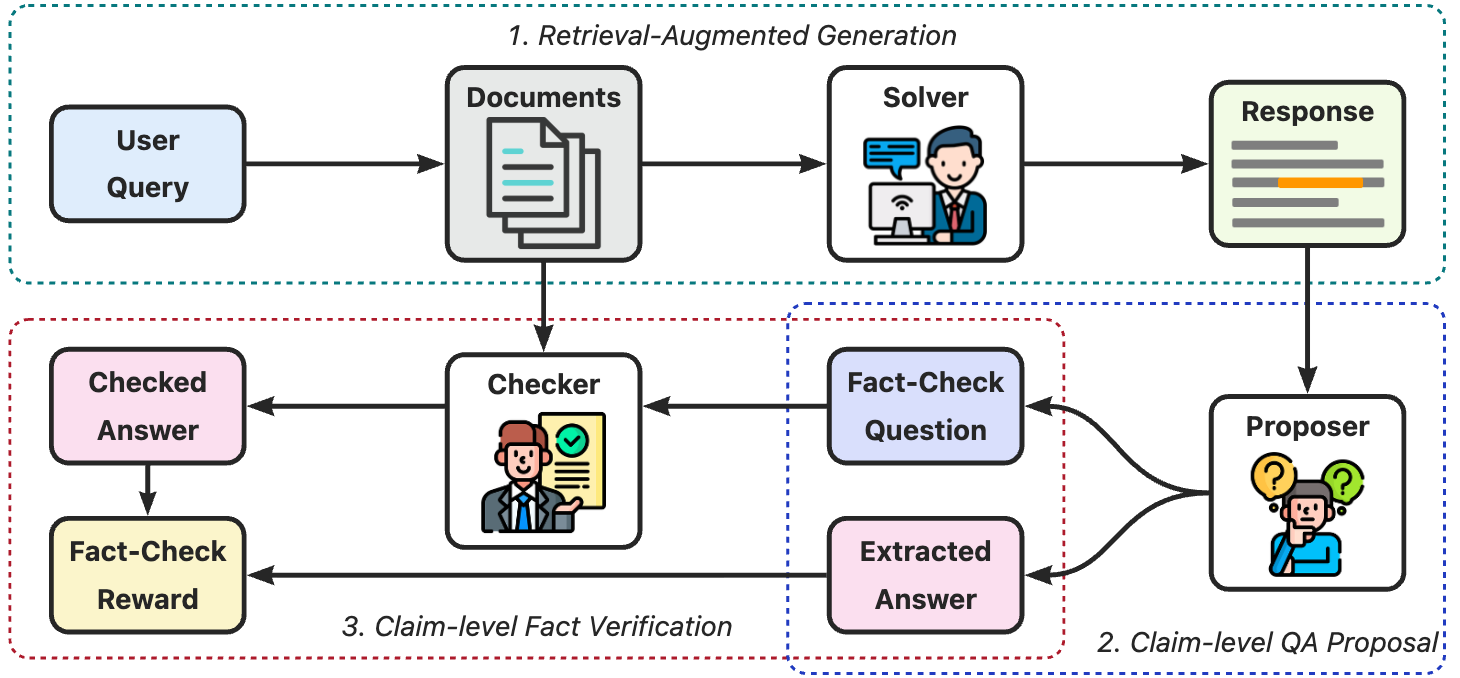
\includegraphics[width=0.88\textwidth]{figures/march-framework-v3.png}
\caption{Overview of the MARCH framework. The \textit{Solver} conducts retrieval-augmented generation base on the input query and related documents. The \textit{Proposer} then decomposes this response into atomic propositions (the orange line in the response block) and formulates verifiable question-answer pairs. The \textit{Checker} performs isolated verification by re-answering questions solely based on the retrieved evidence, without access to the \textit{Solver}’s original output. This information-asymmetric pipeline, where the policy model plays all three roles, is optimized via Multi-Agent Reinforcement Learning (MARL) to achieve robust factual alignment.
%The three agents work in an information-asymmetric scheme for the common goal of correctly validating all the statements. The policy model plays all three characters and self-evolves via the multi-agent reinforcement learning (MARL).
%
%Overview of the MARCH framework. The Solver generates a response based on the query and retrieved documents. The Proposer then decomposes this response into atomic propositions and formulates verifiable question-answer pairs. Finally, the Checker performs isolated verification by re-answering these questions solely based on the retrieved evidence, without access to the Solver’s original output. This information-asymmetric pipeline, where the policy model assumes all three roles, is optimized via Multi-Agent Reinforcement Learning (MARL) to achieve robust factual alignment.
} 
%   By synchronizing generative and grounding signals within a unified optimizer, the policy concurrently refines its narrative synthesis and evidentiary precision, establishing a self-evolving generation and verification loop.}
    \label{fig:framework_1}
\end{figure*}


\section{Introduction}


% Specifically, Reinforcement Learning from Human Feedback (RLHF) \citep{ouyang2022training} typically utilizes monolithic scalar reward models (RMs)~\citep{bradley1952rank} that compress the evaluation of a complex response into a single, coarse-grained preference score, which lacks the resolution to check individual claims or verify granular factual adherence, making a scalar reward an insufficient signal for reinforcing the rigorous evidentiary grounding required in data-intensive tasks. On the other hand, Reinforcement Learning with Verifiable Reward (RLVR)~\citep{deepseekai2025deepseekr1incentivizingreasoningcapability} attempts to provide more objective feedback through external verifiers and LLMs~\citep{liu2025inferencetimescalinggeneralistreward} or deterministic rules~\citep{shao2024deepseekmathpushinglimitsmathematical} and rubrics \citep{gunjal2025rubricsrewardsreinforcementlearning}. However, RLVR is fundamentally constrained by a dual dependency bottleneck: verifiable reward require either expensive, expert-annotated ground-truth that remains scarce in specialized domains, or high-capacity external verifiers whose own reasoning ceilings limit the supervisory signal. Absence of granular verification precludes the model from learning meticulous, document-grounded reasoning through claim-level supervision.

% % 为什么Multi-Agent 可以解？难度有差异，信息是不对称的，合作机制。参考别的paper。核心motivation
% A deeper challenge lies in the scarcity of dense, verifiable training signals for the intermediate steps of document-grounded reasoning. Current RAG supervision remains primarily restricted to outcome-level accuracy, leaving internal reasoning trajectories largely unconstrained~\citep{shi2023replugretrievalaugmentedblackboxlanguage,gekhman2024doesfinetuningllmsnew,yu2024chainofnoteenhancingrobustnessretrievalaugmented,asai2023selfraglearningretrievegenerate}, particularly regarding the interpretation of numerical entities or the reconciliation of disparate evidence. Although post-hoc metrics and external fact verifiers \citep{rashkin2023measuring,gao-etal-2023-rarr,tang2024minicheck} provide utility for evaluation, static verification tools are seldom integrated into the model's internal optimization loop during training. Furthermore, external verifiers often function as black boxes, yielding non-differentiable judgments that resist translation into actionable reinforcement signals, which is further compounded by the full visibility inherent in many current verification schemes. When a verifier possesses complete access to the generated response, the evaluation process becomes susceptible to a priming effect, where the verifier may mirror the generator's internal biases or plausible-sounding factual distortions~\citep{seo2025verifyingverifiersunveilingpitfalls}. Such transparency in the evaluation loop can limit the efficacy of hallucination detection, as the verification stage risks becoming a mere internal consistency check of the narrative rather than a strictly independent audit of the evidence.

Despite the remarkable success achieved by Large Language Models (LLMs)~\citep{openai2024gpt4technicalreport,touvron2023llamaopenefficientfoundation,yang2024qwen2,deepseekai2025deepseekr1incentivizingreasoningcapability,comanici2025gemini25pushingfrontier},
% ,,team2025kimi
the persistence of \emph{hallucinations} remains a fundamental barrier to LLMs' trustworthy usage~\citep{kalai2025language,Huang_2025,ji2023survey,maynez2020faithfulnessfactualityabstractivesummarization}. Even enhanced within Retrieval-Augmented Generation (RAG)~\citep{lewis2020retrieval}, LLMs frequently generate responses that, while linguistically fluent, contradict the provided evidentiary context~\citep{xu2025hallucinationinevitableinnatelimitation}. Such context-conflicting hallucinations~\citep{liu2024lost} are particularly prevalent in data-intensive tasks, manifesting as inaccurate numbers, distorted temporal sequences, or erroneous arithmetic aggregations, even when the source text explicitly contains the requisite information. In high-stakes domains, %~\citep{kang2023deficiency,dahl2024large,kim2025medical},
such as finance~\citep{kang2023deficiency}, law~\citep{dahl2024large}, and healthcare~\citep{kim2025medical}, 
hallucinations are more prohibitive, as users require LLMs to function as meticulous evidence readers rather than creative generators of plausible but unverified narratives.

% SFT本身很难解幻觉，即便Y都是正确的。所以考虑做RL。但是RL的问题也很大，RLVR 怎么样，RLHF怎么样。强调用RL来解是很难的
% In order to mitigate hallucinations in LLMs, Supervised Fine-Tuning (SFT) has been primarily considered as effective~\citep{elaraby2023haloestimationreductionhallucinations,lin2022truthfulqameasuringmodelsmimic,zhou2023limaalignment}. 

Among approaches in mitigating hallucinations, Supervised Fine-Tune (SFT) has been primarily considered as effective~\citep{elaraby2023haloestimationreductionhallucinations,lin2022truthfulqameasuringmodelsmimic,zhou2023limaalignment}. However, several practices emphasize that SFT could also amplify hallucinations by fundamentally operating on behavior cloning~\citep{torabi2018behavioral}, which induces models to prioritize authoritative stylistic patterns over factual accuracy~\citep{casper2023openproblemsfundamentallimitations,zhang2025sirenssongaiocean,gekhman2024doesfinetuningllmsnew}.
% , especially when the target response requires reasoning beyond its internal knowledge ~\citep{casper2023openproblemsfundamentallimitations,zhang2025sirenssongaiocean,gekhman2024doesfinetuningllmsnew}. 
Consequently, Reinforcement Learning (RL) has become a necessity for optimizing LLMs towards more truthfulness
%, specifically under specialized scenarios like RAG
~\citep{yang2025qwen3technicalreport,gemmateam2025gemma3technicalreport}. 
% Yet, the structural properties of standard RL paradigms often clash with the rigorous evidentiary requirements of RAG. 
%However, the low-resolution nature of standard RL reward signals fundamentally clashes with the rigorous evidentiary requirements of RAG in improving fine-grained factual fidelity.
However, the standard outcome-level RL rewards lack the granularity required to supervise fine-grained factual consistency, leading to a fundamental misalignment between the scalar reward and the nuanced evidentiary requirements of RAG.
%
Specifically, Reinforcement Learning from Human Feedback (RLHF) \citep{ouyang2022training} typically relies on reward models (RMs) \citep{bradley1952rank,li2025eliminatinginductivebiasreward,li-etal-2025-aplot,liu2024skyworkrewardbagtricksreward} that compress multifaceted evaluations into coarse-grained scalar scores. This loss of granularity limits the ability to verify individual claims, providing insufficient signals to reinforce the meticulous evidentiary grounding required for data-intensive tasks. Alternatively, while Reinforcement Learning with Verifiable Reward (RLVR) \citep{deepseekai2025deepseekr1incentivizingreasoningcapability} attempts to provide objective feedback via deterministic rules \citep{shao2024deepseekmathpushinglimitsmathematical}, rubrics \citep{gunjal2025rubricsrewardsreinforcementlearning}, or external generalist reward model~\citep{liu2025inferencetimescalinggeneralistreward}, it remains fundamentally constrained by a dual-dependency bottleneck: the scarcity of expert-annotated groundtruth in specialized domains, and the reasoning ceilings of external verifiers. Consequently, unsupported intermediate claims can persist, as models are rewarded for correct final outcomes despite potentially hallucinated reasoning trajectories~\citep{li2025reasoningmodelshallucinatemore}.

%allows unsupported intermediate claims to persist while rewarding the model for correct outcomes despite hallucinated trajectories

%Moreover, current RAG hallucination research primarily focuses on outcome-level supervision~\citep{shi2023replugretrievalaugmentedblackboxlanguage, gekhman2024doesfinetuningllmsnew,asai2023selfraglearningretrievegenerate,yu2024chainofnoteenhancingrobustnessretrievalaugmented}, leaving internal trajectories largely unconstrained. 
While post-hoc metrics and fact-checkers \citep{tang2024minicheck,rashkin2023measuring,gao-etal-2023-rarr,baker2025monitoringreasoningmodelsmisbehavior,guan2025monitoringmonitorability} provide utility for evaluation, such static tools are seldom integrated into the internal optimization loop to provide actionable, claim-oriented guidance. More critically, the efficacy of such verifiers is fundamentally undermined by the 
% \textit{information symmetry} 
\textit{information leakage} inherent in current evaluation schemes \citep{seo2025verifyingverifiersunveilingpitfalls}. 
% Specifically, a verifier is susceptible to a \textit{priming effect} when granted full visibility of the generated response, risking a mere validation of internal consistency rather than a strictly independent grounding against the source evidence. Consequently, the lack of an independent, claim-level scrutiny prevents LLM from internalizing the meticulous, document-anchored reasoning necessary for factual precision.
Specifically, concurrent exposure to the query, documents, and generated response induces a confirmation bias~\citep{sharma2025understandingsycophancylanguagemodels}. In this state, verifiers tend to prioritize validating internal coherence over objective grounding against source evidence, leading to the unwarranted endorsement of erroneous claims. This compromised ``blind scrutiny'' prevents the model from internalizing the rigorous, document-anchored reasoning essential for high-fidelity generation.

%as the blind scrutiny essential for factual precision is compromised. Consequently, the model fails to internalize the rigorous, document-anchored reasoning required for high-fidelity generation.


%Specifically, concurrent exposure to the query, documents, and the model's own response induces a strong self-confirmation bias. In this state, verifiers tend to prioritize internal coherence over objective grounding against source evidence, leading to the unwarranted endorsement of erroneous claims.

To address above factuality challenges, we introduce \textbf{M}ulti-\textbf{A}gent \textbf{R}einforced self-\textbf{C}heck for \textbf{H}allucination (MARCH), an RL-based framework that enforces factual alignment through deliberate information asymmetry. 
MARCH orchestrates a collaborative pipeline of three specialized agents: a \textit{Solver}, a \textit{Proposer}, and a \textit{Checker}, to prevent model-based verifiers from taking cognitive shortcuts through confirmation bias.
%
%an RL-based framework that mitigates RAG hallucinations through the strategic exploitation of information asymmetry collaboration that prevents verifiers from taking shortcuts through internal consistency checks among three specialized agents: a {Solver}, a {Proposer}, and a {Checker}.
%As shown in Figure~\ref{fig:framework_1}, the Solver initiates the training by generating a response based on retrieved documents given the input query. Subsequently, the {Proposer} serves as a Response Atomizer, deconstructing the {Solver’s} narrative into a set of discrete, numerically-grounded questions whose answers are explicitly contained within the generated text. Finally, the {Checker} is tasked with answering these questions by relying exclusively on the original documents, remaining strictly blinded to the {Solver’s} narrative to prevent cognitive contamination. Through an asymmetric decoupling, MARCH transforms generation-verification into a rigorous cross-examination between the Solver's claims and the source evidence, rather than a circular confirmation of plausible text. 
%
As illustrated in Figure~\ref{fig:framework_1}, the Solver first generates a response based on the query and retrieved documents. Subsequently, the Proposer acts as a 'Response Atomizer,' deconstructing the narrative into discrete, verifiable claims. Finally, the Checker validates these claims by re-answering them exclusively based on the source documents, strictly blinded to the Solver’s original output to avoid cognitive contamination. Through this asymmetric decoupling, MARCH transforms the verification process from a circular confirmation of plausible text into a rigorous cross-examination between generated claims and factual evidence.
%
%
%During training, MARCH achieves agentic self-evolution through a zero-tolerance reward mechanism: any discrepancy between the {Proposer’s} extracted claims and the {Checker’s} document-based findings triggers a binary penalty on the entire reasoning trajectory, which ensures agents' outputs are strictly anchored in verified evidence, thereby internalizing the capability of rigorous reasoning and self-verification.
During training, MARCH promotes agentic self-evolution via a zero-tolerance reward mechanism: any discrepancy between the Proposer’s extracted claims and the Checker’s document-based validation triggers a penalty on the entire response trajectory. This encourages the agents to align their outputs strictly with retrieved evidence, effectively internalizing the capability for rigorous, document-anchored statements.
% Through the asymmetric and collaborative interaction, the system systematically internalizes reasoning and self-verification trajectories. 
%Experimentally, MARCH yields a significant reduction in hallucination compared to the base model without the necessity for annotations or an external fact-checker, demonstrating the efficacy of asymmetric collaborative reinforcement. Furthermore, MARCH enables an 8B-parameter LLM to achieve performance parity with leading closed-source LLMs on hallucination benchmarks while yielding substantial gains in general RAG-QA tasks, establishing a scalable and verifiable pathway toward trustworthy agentic training.
%
Experimentally, MARCH achieves a substantial reduction in hallucinations compared to its base model, without requiring additional human annotations or external fact-checking tools, thereby demonstrating the efficacy of our asymmetric collaborative reinforcement paradigm. Notably, an 8B-parameter LLM equipped with MARCH achieves performance parity with leading closed-source models on multiple hallucination benchmarks, while simultaneously delivering significant gains in general RAG-QA tasks. These results establish a scalable and verifiable pathway toward trustworthy, agentic self-improvement for large language models.

% \begin{figure*}[htbp!]
    % \centering
    % \includegraphics[width=0.9\textwidth]{figures/fc_framework1.pdf}
% \caption{Overview of our self-play multi-agent framework. A shared LLM policy is instantiated as three interactive agents: a \textit{Solver}, a \textit{Proposer}, and a \textit{Checker}. Given a user query and retrieved documents, the \textit{Solver} generates a long-form response. The \textit{Proposer} then operates in self-play on the generation, extracting key numeric claims and converting them into auxiliary factual questions with self-answers. These questions, together with the retrieved documents, are passed to the \textit{Checker}, which performs document-grounded answering by re-answering the questions using only the docs. A separate fact-check reward module compares the \textit{Proposer’s} self-answers with the \textit{Checker’s} doc-grounded answers and aggregates the agreement into a fact-check reward signal that jointly trains the \textit{Solver} and the \textit{Checker}, encouraging doc-consistent generation and reliable document-grounded verification.}
    % \label{fig:framework_1}
% \end{figure*}

% \section{Preliminaries}
% \paragraph{LLM as a policy Agent.} We treat an LLM $\pi_\theta$ as an autonomous agent parameterized by $\theta$. Given a user query $\vx$, the agent $\pi_\theta$ generates a response $\vy\sim\pi_{\theta}(\cdot\mid\vx)$, where each token $y_t$ is sampled from the vocabulary $\mathcal{V}$ according to the conditional probability $\pi_\theta(y_t \mid \vx, \vy_{<t})$.

% \paragraph{Reinforcement Learning from Human Feedback (RLHF).} RLHF has become one of the essential training processes to align LLMs with human values~\citep{ouyang2022traininglanguagemodelsfollow}. With a well-learned reward model (RM) $r(\cdot)$ scoring the degree of human preference of generated response $\vy \in \gY$ given input prompt $\vx \in \gX$, RLHF optimizes the LLM policy $\pi_\theta(\vy\mid\vx)$  with the follow objective: 
% \begin{equation}\label{eq:RLHF}
%     \mathbb{E}_{\vx\sim \mathcal{X},\vy\sim\pi_\theta(\cdot\mid\vx)} \Big[ r(\vx, \vy) - \beta\cdot\text{KL}[\pi_\theta(\vy\mid\vx)\Vert\pi_\text{ref}(\vy\mid\vx)]\Big],
% \end{equation}
% where $\pi_\text{ref}(\vy \mid \vx)$ is the initial model policy served as a reference, $\beta > 0$ controls the strength of a Kullback-Leibler (KL) divergence~\citep{csiszar1975divergence} between the reference model $\pi_\text{ref}(\vy\mid\vx)$ and the learning policy $\pi_\theta(\vy\mid\vx)$. 

% \paragraph{Proximal Policy Optimization (PPO).} To train an LLM $\pi_\theta$ with \eqref{eq:RLHF}, Proximal Policy Optimization (PPO) \citep{schulman2017proximalpolicyoptimizationalgorithms} has been recognized as the mainstream optimization approach~\citep{openai2024gpt4technicalreport,bai2023qwentechnicalreport,rafailov2024direct}, which utilizes a clipped surrogate loss $\mathcal{L}$ to constrain the policy updates:
% \begin{equation}
% \mathcal{L}(\theta) = {\mathbb{E}}_t \left[ \min \left( r_t(\theta) \hat{A}_t, \text{clip}(r_t(\theta), 1-\epsilon, 1+\epsilon) \hat{A}_t \right) \right],
% \end{equation}
% where $r_t(\theta)$ denotes the probability ratio between the current and previous policies and $\epsilon$ is a clip coefficient. The term $\hat{A}_t$ represents the estimated advantage computed by Generalized Advantage Estimator (GAE) \citep{schulman2015high}.

% \subsection{Multi-Agent Reinforced Check Design}\label{met:motivation}
% The fundamental challenge in optimizing \eqref{eq:oracle_objective} lies in the absence of dense, high-quality ground-truth $\mathcal{A}^*$. 

% While these agents cooperate to complete the generation and factual verification pipeline, a naive implementation often suffers from {reward hacking} due to {information symmetry}. If the Checker shares the Solver's full narrative context, it potentially tends to simply mirror the Solver's claims rather than rigorously scrutinizing the source documents. To mitigate this bias, we introduce a physical {information barrier} that strictly blinds the Checker to the Solver’s response, which transforms the collaboration into an {asymmetric play}: the Solver attempts to maximize narrative utility, while the blinded Checker acts as a static adversary that only grants rewards upon a successful {independent reconstruction} of facts. Consequently, our framework represents a form of asymmetric collaboration driven by structural tension, forcing the shared policy $\pi_\theta$ to maintain factual identity across asymmetric information states and preventing the degenerate ``mirroring'' collapse common in traditional self-correction.

\section{Methodology}
\subsection{Problem Formulation and Overview}
Given an input query $\vx \in \gX$ and a set of retrieved documents $\mD = [\vd_1, \vd_2, \dots, \vd_l]$, we aim to optimize a policy model $\pi_{\theta}(\vy|\vx, \mD)$ that generates a response $\vy$ with maximum factual grounding aligned with the provided evidences in $\mD$. Formally, suppose we can extract all the statements of facts $\{\va_1,\va_2,\dots,\va_n\}$ from the response $\vy$ using a function $\gA(\cdot)$, as $\gA(\vy) = \{\va_i\}_{i=1}^n$. Then, from the perspective of reinforcement learning with verifiable reward (RLVR), if an oracle set of ground-truth annotations $\mathcal{A}^* = \{\va^*_1, \dots, \va^*_n\}$ is ideally available for every atomic statement $\va_i$ in $\vy$, the optimization objective is to maximize the expected evidentiary consistency:
\begin{equation}\label{eq:oracle_objective}
   \max_{\theta} \mathbb{E}_{\vx\sim \gX, \vy \sim \pi_{\theta}(\cdot | \vx, \mD)} [ R(\{\va_i, \va^*_i\}_{i=1}^n) ],
\end{equation}
where $R(\cdot)$ is a fact-check function that identifies the exact match between $\mathcal{A}(\vy) = \{\va_i\}_{i=1}^n$ and $\{\va^*_i\}_{i=1}^n$. However, $\mathcal{A}^*$ is practically unavailable in most application domains and requires enormous human annotation. 

Therefore, we reformulate \eqref{eq:oracle_objective} into a self-contained, verifiable objective by decomposing the grounding process into three separate agent tasks, as illustrated in Figure~\ref{fig:framework_1}: 
\begin{enumerate}[leftmargin=2.5ex]
\vspace{-1mm}
    \item \textbf{Response Generation}: a Solver agent ordinarily responses $\vy$ based on the input query $\vx$ and retrieved context $\mD$. 
    \item  \textbf{Claim-level QA Proposal}: a Proposer agent decomposes the response $\vy$ into $n$ discrete factual claims in a question-answering (QA) format, as $\gQ(\vy) = \{(\vq_i, \va_i)\}_{i=1}^n$.
    \item \textbf{Factual Verification}: a Checker agent answers all the atomic questions $\{\vq_i\}_{i=1}^n$ as $\{\hat{\va}_i\}_{i=1}^n$ with only the retrieval documents $\mD$ provided, without any access to the original response $\vy$ and extracted answers$\{\va_i\}_{i=1}^n$. %  to produce $\bm{\lambda}$ consisting reference answers $\{\hat{\va}_i\}_{i=1}^n$ and the corresponding justifications.
\end{enumerate}
%(1) {Response Generation} that synthesizes a narrative $\vy$ from the query $\vx$ and retrieved context $\mD$. (2) {Claim Atomization} that decomposes the continuous narrative $\vy$ into $n$ discrete factual units $\mathcal{Q} = \{(\vq_i, \va_i)\}_{i=1}^n$ with respect to $\vx$. (3) {Independent Grounding} that performs a blinded grounding of these units against $\mD$ to produce $\bm{\lambda}$ consisting reference answers $\{\hat{\va}_i\}_{i=1}^n$ and the corresponding justifications. 
%A detailed illustration of the above task decomposition is in Figure~\ref{fig:framework_1}. 
By substituting the unreachable oracle $\va^*_i$ with the  grounding result $\hat{\va}_i$ from the multi-agent pipeline, we approximate the factuality optimization as: % {MARCH Integrated Objective} \pengyu{need revise}:
\begin{equation}\label{eq:integrated_objective_vanilla}
   \max_{\theta} \mathbb{E}_{\vx\sim \gX, \vy \sim \pi_{\theta}(\cdot | \vx, \mD)} \left[ R(\{(\va_i, \hat{\va}_i)\}_{i=1}^n) \right].
\end{equation}
By optimizing \eqref{eq:integrated_objective_vanilla}, we force $\pi_\theta$ to internalize a rigorous verification logic, ensuring that the generated content is strictly anchored in the source evidence to enhance overall factual accuracy. We call the proposed learning scheme \textbf{M}ulti-\textbf{A}gent \textbf{R}einforced self-\textbf{C}heck for \textbf{H}allucination (MARCH).




\subsection{MARCH Modeling}\label{met:modeling}

As shown in Figure~\ref{fig:framework_1}, we instantiate the functional primitives identified above into three specialized agents derived from the same base policy $\pi_\theta$: a \textit{Solver}, a \textit{Proposer}, and a \textit{Checker}, which are conditioned to exhibit distinct epistemic behaviors, effectively transforming the RAG task into a structured, asymmetric cooperative game. MARCH begins with the {Solver}'s policy:
\begin{equation}
%\small
%    \vy \sim \nu_\text{solve}(\cdot | \vx, \mD) \equiv \pi_{\theta}(\cdot | \vx, \mD, \text{Solver-Prompt}).
   \nu_{\text{solve}}(\cdot | \vx, \mD)  =  \pi_{\theta}(\cdot | \vx, \mD,  \vs_\text{solve}),
\end{equation} where $\vs_\text{solve}$ is the Solver's system prompt (as shown in Appendix~\ref{app:answer_prompt}) to induce the policy model $\pi_\theta$ to generate a comprehensive response $\vy$ given the retrieval documents $\mD$ and the input $\vx$.

To decouple the continuous response $\vy$ into verifiable components, the {Proposer} agent functions as a \textit{Response Atomizer} that bridges narrative synthesis and discrete verification:
\begin{equation}
  \nu_{\text{propose}}(\cdot | \vy) = \pi_{\theta}(\cdot|  \vy, \vs_\text{propose}),
\end{equation}
where the Propser's system prompt $\vs_\text{propose}$ is in Appendix~\ref{app:propose_qa}.
Specifically,  $\nu_{\text{propose}}$ decomposes the response $\vy$ into a set of $n$ self-contained factual question-answer (QA) pairs $\mathcal{Q}(\vtau) = \{(\vq_i, \va_i)\}_{i=1}^n$, where each $\vq_i$ represents a targeted inquiry,  and each $\va_i$ denotes the corresponding claim asserted in $\vy$. The function $\gQ(\cdot)$ extracts the QA pairs from the Proposer's generation $\vtau \sim \nu_\text{propose}(\cdot|\vy)$.  % The atomization produced by $\nu_{\text{proposer}}$ ensures that every semantic leap within the Solver's response is mapped to a granular, verifiable unit by:
% \begin{equation}
%  \{(\vq_i, \va_i)\}_{i=1}^n \sim \boldsymbol{\tau},\quad s.t.\quad \boldsymbol{\tau}\sim
% \end{equation}
the {Checker} operates as the \textit{Blinded Auditor} and the linchpin of the asymmetric cooperation:
\begin{equation}
    \nu_{\text{check}}(\cdot |\{\vq_i\}_{i=1}^n, \mD) = \pi_{\theta}(\cdot| \{ \vq_i\}, \mD, \vs_\text{check})
\end{equation}
with the Checker's prompt $\vs_\text{check}$ in Appendix~\ref{app:check_qa}
To eliminate confirmation bias and break information symmetry, when tasked with answering $\vq_i$,  $\nu_{\text{check}}$ is strictly {blinded} to the Solver's response $\vy$ and the corresponding claims $\va_i$. %Guided by \textit{Checker-Prompt}~\ref{app:check_qa}, 
%
the \textit{Checker} replies all the queries $\{ \vq_i\}_{i=1}^n$ in a response $\bm{\lambda}\sim \nu_\text{check}(\cdot|\{\vq_i\}_{i=1}^n, \mD)$, only based on the RAG documents $\mD$. The corresponding answers $\gA(\bm{\lambda}) = \{\hat{\va}_i\}_{i=1}^n$ are parsed by the function $\gA(\cdot)$ to serve as the re-checked answers to the QA pairs $\{(\vq_i, \va_i)\}_{i=1}^n$.
% \begin{equation}
% \begin{aligned}
% \small
%    & \{\hat{\va}_i\}_{i=1}^n\sim\bm{\lambda},\quad
%     s.t.\quad\bm{\lambda} \sim  
% \end{aligned}
% \end{equation}

\paragraph{Overall Objective.} By integrating the conditional dependencies of the \textit{Solver},  the \textit{Proposer}, and the \textit{Checker}, MARCH defines a unified {asymmetric cooperative and play objective} by focusing on the {evidentiary identity} between \textit{Solver's} response $\vy$ and \textit{Checker's} independent grounding trajectory $\bm{\lambda}$, mediated by the atomic claim decomposition of the \textit{Proposer}. The optimization goal is to maximize the expected reward based on the consistency of claims, marginalized over the discrete atomization performed by $\nu_\text{propose}$:
\begin{align}
   &\max_{\pi_\theta}\ \mathbb{E}_{
   \vx\sim\gX, \vy \sim \nu_{\text{solve}} (\cdot|\vx, \mD)} \left[ R(\{(\va_i, \hat{\va}_i)\}_{i=1}^n) \right] \label{eq:integrated_objective} \\
\text{s.t. }
   \{(\vq_i, \va_i)\}_{i=1}^n = \gQ(\vtau)&, \ \vtau\sim \nu_{\text{propose}}(\cdot|\vy) \{\hat{\va}_i\}_{i=1}^n = \gA(\bm{\lambda}),   \ \bm{\lambda} \sim \nu_{\text{check}}(\cdot|\{\vq_i\}_{i=1}^n, \mD)  \nonumber
\end{align}   
%
% \begin{equation}\label{eq:integrated_objective}
% \small
%    \max_{\theta} \mathbb{E}_{\substack{
%    \vx\sim\gX, \vy \sim \nu_\text{solve} (\cdot|\vx, \mD),\\
%    \{(\vq_i, \va_i)\}_{i=1}^n \sim \nu_\text{propose}(\cdot|\vy),\\
%    \bm{\lambda} \sim \nu_\text{check}(\cdot|\{\vq_i\}_{i=1}^n, \mD),\{\hat{\va}_i\}_{i=1}^n\sim\bm{\lambda}}} \left[ R(\{(\va_i, \hat{\va}_i)\}_{i=1}^n) \right],
% \end{equation}
% where $R(\{(\va_i, \hat{\va}_i)\}_{i=1}^n)$ denotes a discrete reward function that outputs a score based on the identity match between each \textit{Solver’s} asserted claim $\va_i$ and the \textit{Checker’s} independent answer $\hat{\va}_i$. By optimizing \eqref{eq:integrated_objective}, we force the shared policy $\pi_\theta$ to synchronize its generation and auditing capabilities, ensuring that the Solver's narrative synthesis is strictly bounded by the Checker's evidentiary discovery. By updating $\pi_\theta$ using both the Solver's reasoning paths and the Checker's audit trajectories, the model internalizes a self-consistent verification loop without the need for external supervision.
where $R(\cdot)$ measures the evidentiary identity between each asserted claim $\va_i$ and the independent grounding $\hat{\va}_i$. By optimizing \eqref{eq:integrated_objective}, the policy $\pi_\theta$ is compelled to internalize a rigorous verification logic, ensuring that its narrative synthesis is strictly anchored in verifiable evidence to enhance overall factual accuracy, which also develops a self-consistent grounding capability that eliminates reliance on external supervision.


\subsection{MARCH Implementation}\label{met:implementation}
In our implementation, we specifically prioritize {numerical and quantitative verification}, driven by the observation that in data-intensive RAG scenarios, LLMs frequently suffer from hallucinations such as misquoting figures or altering numerical values during context integration. By anchoring the verification loop on these high-fidelity tokens, MARCH provides a more rigorous evidentiary baseline for grounding long-form reasoning.
\paragraph{Zero-Tolerance Reward (ZTR).}
To enforce absolute factual grounding, we define a binary {Zero-Tolerance Reward} function $R(\{(\va_i, \hat{\va}_i)\}_{i=1}^n)$ in \eqref{eq:integrated_objective}. In the RAG context, we posit that any single hallucinated claim $\va_i$ within the response $\vy$ invalidates the entire reasoning chain. Therefore, a trajectory is assigned a successful score only if every claim $\va_i$ asserted by the \textit{Solver} achieves an identity match with the consensus answer $\hat{\va}_i$ extracted by the \textit{Checker}:
\begin{equation}\label{eq:ztr_reward}
%\small
    R(\{(\va_i, \hat{\va}_i)\}_{i=1}^n) = 
    \begin{cases} 
    0, \hspace{-1.5ex}&\text{if every } \va_i = \hat{\va}_i %\in \{1, \dots, n\} 
    \\
    -1, \hspace{-1.5ex}&\text{otherwise}
    \end{cases}
\end{equation}
%
% \begin{equation}\label{eq:ztr_reward}
% %\small
%     R(\{(\va_i, \hat{\va}_i)\}_{i=1}^n) = 
%     \begin{cases} 
%     0,&\text{if } \va_i = \hat{\va}_i,  \forall i \in \{1, \dots, n\} \\
%     -1,&\text{otherwise}
%     \end{cases}
% \end{equation}
%
This ``all-or-nothing'' reward structure prevents the policy $\pi_\theta$ from optimizing for partial correctness or stylistic plausibility, forcing the model to prioritize strict evidentiary identity. Besides, to ensure the \textit{Checker} provides a reliable baseline for the audit and to reduce the variance of the reward signal, we employ a multi-sampling strategy during the cross-validation phase. For each question $\vq_i$ generated by the \textit{Proposer},  $\nu_\text{check}$ generates multiple independent audit trajectories. We apply a majority voting to determine the final consensus answer $\hat{\va}_i$, which effectively mitigates stochastic errors in \textit{Checker's} generation in one independent audit.
\paragraph{Policy Optimization.}
We optimize the shared policy $\pi_\theta$ of the three agents using Proximal Policy Optimization (PPO) \citep{schulman2017proximalpolicyoptimizationalgorithms}. 
Critically, we incorporate both the reasoning path $\vy$ and the audit trajectory $\bm{\lambda} \sim \nu_\text{check}(\cdot|\{\vq_i\}, \mD)$ into the optimization loop, ensuring that $\pi_\theta$ concurrently evolves as both a reliable generator and a rigorous auditor.
% By refining the audit trajectory in addition, the policy internalizes a more precise evidentiary baseline, which in turn provides higher-quality feedback for the reasoning path.
Consequently, each original query of a training batch $\vx_i \in \mathcal{B}$ contributes two distinct reward signals to the policy, allowing $\pi_\theta$ to learn the fine-grained correspondence between narrative synthesis and independent document-grounding within a unified training batch. While both trajectories derive their terminal reward from the same evidentiary identity match (\eqref{eq:ztr_reward}), corresponding advantages $\hat{A}$ and KL-divergence~\citep{csiszar1975divergence} penalties against the reference model $\pi_\text{ref}$ are estimated independently. The joint gradient is computed as the sum of gradients across all individual trajectories $\nabla_\theta \mathcal{L}_{\text{MARCH}}(\theta) \approx$
%
\begin{align}\label{eq:expanded_gradient}
    \frac{1}{2|\gB|} \sum_{\vx \in \mathcal{B}} \Bigg[\sum_{t=1}^{|\vy|} \hat{A}_{y}^t  \nabla_\theta \log \pi_\theta({y}^t | \cdot)  +\sum_{t=1}^{|\bm{\lambda}|} \hat{A}_{\lambda}^t   \nabla_\theta \log \pi_\theta({\lambda}^t | *)
    - \beta \nabla_\theta \text{KL}[\pi_\theta \| \pi_{\text{ref}}] \Bigg]
\end{align}
% \begin{equation}\label{eq:expanded_gradient}
% \begin{aligned}
%     \frac{1}{2|\mathcal{B}|} \sum_{i \in \mathcal{B}} \sum_{\tau' \in \{\vy_i, \bm{\lambda}_i\}} \Big[ & \sum_{t=1}^{|\bm{\lambda}|} \nabla_\theta \log \pi_\theta({\lambda}^t | \cdot) \hat{A}_{\lambda}^t \\
%     & - \beta \cdot \nabla_\theta \text{KL}[\pi_\theta \| \pi_{\text{ref}}] \Big]
% \end{aligned}
% \end{equation}
where $\hat{A}_\lambda^t$  and  $\hat{A}_y^t$ are the $t$-th token's corresponding advantages of the Checker's output $\bm{\lambda}$ and the Solver's output $\vy$, estimated via Generalized Advantage Estimation~\citep{schulman2015high}. The notation $(\cdot)$ and $(*)$ in \eqref{eq:expanded_gradient} encapsulates the respective contexts for brevity: $(\vx, \mD, \vy^{<t})$ and $(\{\vq_i\}, \mD, \bm{\lambda}^{<t})$ for the Solver's and the Checker's generation prefixes. \eqref{eq:expanded_gradient} ensures that $\pi_\theta$ concurrently refines its narrative generation and evidentiary precision, internalizing a self-contained verification loop where generative assertions are inherently tethered to the policy's own auditing capacity. We summarize our training algorithm in Algorithm~\ref{alg:training}.

\begin{algorithm*}[!t]
\textbf{Input}: An LLM Policy $\pi_\theta$; A Training Batch $\mathcal{B}=\{(\vx_i,\mD_i)\}_{i=1}^{|\mathcal{B}|}$; Solver, Proposer and Checker System Prompts $\{\vs_{\text{solve}}, \vs_{\text{propose}}, \vs_{\text{check}}\}$\;
\tcp{Phase 1: Multi-Agent Collaboration and Rollout}
\For{each training sample $(\vx, \mD) \in \mathcal{B}$}{
    \tcp{Step 1: Generate reasoning path $\vy$ from Solver}
    Sample $\vy \sim \nu_{\text{solve}}(\cdot\mid\vx,\mD) = \pi_{\theta}(\cdot | \vx, \mD, \vs_{\text{solve}})$\;
    
    \tcp{Step 2: Atomize response $\vy$ by Proposer and Parse QA pairs by $\mathcal{Q}(\cdot)$}
    Sample $\boldsymbol{\tau}\sim\nu_{\text{propose}}(\cdot\mid\vy) = \pi_{\theta}(\cdot \mid \vy, \vs_{\text{propose}})$\;
    Extract QA pairs $\{(\vq_i,\va_i)\}_{i=1}^{n}=\mathcal{Q}(\boldsymbol{\tau})$\;
    
    \tcp{Step 3: Generate audit trajectory $\bm{\lambda}$ from Checker and Parse re-checked answers by $\mathcal{A}(\cdot)$}
    Sample $\bm{\lambda}\sim\nu_{\text{check}}(\cdot\mid\{\vq_i\}_{i=1}^n,\mD) = \pi_{\theta}(\cdot \mid \{\vq_i\}_{i=1}^n,\mD, \vs_{\text{check}})$\;
    Parse re-checked answers $\{(\hat{\va}_i)\}_{i=1}^{n}=\mathcal{A}(\bm{\lambda})$\;
    
    \tcp{Step 4: Unified reward labeling}
    Calculate Zero-Tolerance Reward $R_i$ by \eqref{eq:ztr_reward} (based on the match between $\va$ and $\hat{\va}$)\;
    
    \tcp{Step 5: Store both reasoning and auditing trajectories}
    Add $\vy_i$ and $\bm{\lambda}_i$ to the unified batch trajectory set $\mathcal{T}_{\mathcal{B}}$\;
    Associate both $\vy_i$ and $\bm{\lambda}_i$ with terminal reward $R_i$\;
}

\tcp{Phase 2: Joint Policy Optimization}
\For{each trajectory $\tau' \in \mathcal{T}_{\mathcal{B}} = \{\vy_i, \bm{\lambda}_i\}$}{
    Estimate Advantage $\hat{A}_{\tau'}$ using GAE based on $R_i$\;
    Compute ${\text{KL}}(\pi_\theta \| \pi_{\text{ref}})$ for each token in $\tau'$\;
}
Update $\pi_\theta$ by computing the joint gradient $\nabla_\theta \mathcal{L}_{\text{MARCH}}(\theta)$ according to \eqref{eq:expanded_gradient}\:
$    \frac{1}{2|\gB|} \sum_{\vx \in \mathcal{B}} \Bigg[\sum_{t=1}^{|\vy|} \hat{A}_{y}^t  \nabla_\theta \log \pi_\theta({y}^t | \cdot) +\sum_{t=1}^{|\bm{\lambda}|} \hat{A}_{\lambda}^t   \nabla_\theta \log \pi_\theta({\lambda}^t | *) - \beta \nabla_\theta \text{KL}[\pi_\theta \| \pi_{\text{ref}}] \Bigg]$\;
where the notation $(\cdot)$ and $(*)$ in \eqref{eq:expanded_gradient} encapsulates the respective contexts for brevity: $(\vx, \mD, \vy^{<t})$ and $(\{\vq_i\}, \mD, \bm{\lambda}^{<t})$ for the Solver's and the Checker's generation prefixes\;
\caption{MARCH Training Process.}
\label{alg:training}
\end{algorithm*}

% \paragraph{Self-Play Mechanism for LLMs.} Originating from TD-Gammon~\citep{tesauro1995temporal}, the concept of self-play has a long history in achieving superhuman performance in strategic games like Alpha-Go~\citep{silver2016mastering} and Alpha-Zero~\citep{silver2017mastering}, with the central idea of training the model by playing against its previous version for progressive improvements. Recently, self-play fine-tuning has successfully boosted LLMs in a series of subsequent works, including alignment~\citep{chen2024self,wu2024self}, instruction following~\citep{dong2024self,cheng2024spar}, theorem proving~\citep{dong2025stp}, reasoning~\citep{cheng2024self,zhao2025absolute}, and tool-use~\citep{lu2025search,xu2025acesearcher}. Distinct from these self-play paradigms, our method focuses on enforcing internal factual accountability within a single policy rather than iterative model-level competition. By instantiating generative and evaluative roles separated by a structural information barrier, we synthesize numerically-grounded rewards to penalize logical discrepancies, compelling the model toward strict evidentiary adherence.

\section{Experiment}
We first evaluate the effectiveness of MARCH in mitigating hallucinations.
% and improving factual adherence to retrieved evidence. 
Then, we show that the improved factual consistency ability helps downstream reasoning tasks like Question-Answering.
% In this section, we empirically evaluate our self-play multi-agent framework from two perspectives: (i) its ability to improve factual consistency detection and adherence to retrieved evidence, and (ii) the downstream gains on question answering performance brought by improved factual behavior. 
% We conduct experiments under multiple settings to answer the following questions:
% \begin{itemize}
%     \item \textbf{RQ1:} Does our framework improve the model's ability to detect and penalize factual inconsistencies with respect to retrieval documents?
%     \item \textbf{RQ2:} Does better fact-checking and document-following behavior bring better reasoning ability on complex multi-hop QA tasks?
%     \item \textbf{RQ3:} How robust is the method across different base LLMs, datasets, and types of numerical or factual reasoning?
% \end{itemize}
\subsection{Training Setup}
\paragraph{Training Datasets and Base Model.}
We train our framework covering: a {STEM} (Science-Technology-Engineering-Math) setting based on BioASQ~\citep{krithara2023bioasq}, and a {General} setting based on 2WikiMultiHopQA~\citep{ho2020constructing} and MuSiQue~\citep{trivedi2022musique}. Crucially, training is performed using only queries and retrieved documents, without access to ground-truth answers or annotations. Table~\ref{tab:training_datasets_stats} shows the number of retrieved documents per query and the document lengths vary widely across datasets, and a substantial fraction of the documents are irrelevant to the query (e.g., 30.1\% for STEM and up to 88.4\% for MuSiQue). Such a high level of noise and heterogeneity in the retrieval docs makes the training setting highly realistic but also extremely challenging, as the agents must learn to perform document-grounded fact checking in the presence of many noisy documents. We consider Meta-Llama3.1-8B-Instruct~\citep{touvron2023llamaopenefficientfoundation} as the initialization policy.


\begin{table*}[!h]
\centering
\caption{Statistics of the training dataset, where we report the number of training samples, average query length, the number of retrieved documents per query, the average document length, and the proportion of documents that are irrelevant to the query. The large variance in document counts and lengths, together with the high ratio of irrelevant documents, highlights the realism and difficulty of our training setup.}
\resizebox{\textwidth}{!}{
\begin{tabular}{ccccccccccc}
\toprule
\multirow{2}{*}{Dataset} & \multirow{2}{*}{Original Dataset} & \multirow{2}{*}{\#Samples} & \multirow{2}{*}{Avg. Query Len} & \multicolumn{3}{c}{\#Docs per Query} & \multicolumn{3}{c}{Total Doc Len (words)} & \multirow{2}{*}{Irrelevant Doc Ratio} \\ 
 &  &  &  & Avg & Max & Min & Avg & Max & Min &  \\ \midrule
STEM & BioASQ & 4721 & 8.62 & 9.03 & 157 & 1 & 1314.86 & 22135 & 1 & 30.14\% \\ \midrule
\multirow{2}{*}{General} & 2WikiMultiHopQA & 4500 & 12.87 & 10 & 10 & 10 & 575.65 & 2099 & 95 & 24.4\% \\
 & MuSiQue & 4500 & 15.85 & 19.99 & 20 & 16 & 11221.72 & 20741 & 4112 & 88.35\% \\ \bottomrule
\end{tabular}
}\label{tab:training_datasets_stats}
\end{table*}


\paragraph{Training Details.}
Training framework is built upon the \texttt{VerL}~\citep{Sheng_2025}, and we employ Fully Sharded Data Parallel (FSDP)~\citep{zhao2023pytorchfsdpexperiencesscaling} for efficient multi-node multi-GPU training. During the training rollout, we utilize the \texttt{vLLM}~\citep{kwon2023efficientmemorymanagementlarge} for efficient sample generation with the temperature of 0.6. The PPO~\citep{schulman2017proximalpolicyoptimizationalgorithms} training is conducted for a single epoch with a global batch size of 32, with a max prompt length of 24,567, max response length of 8,192. We set learning rates for the actor and the critic as $1\times10^{-6}$ and $1\times10^{-5}$, respectively. We save and evaluate a checkpoint every 20 steps, and report results from the single best-performing checkpoint selected based on the highest average score across all evaluation benchmarks. More detailed training hyper-parameters are in Appendix~\ref{app:training_hp}.

% \paragraph{Evaluation Metrics.} Unless otherwise specified, we adopt an {LLM-as-a-judge} protocol by using Qwen3-235B-A22B~\citep{yang2025qwen3technicalreport} and report response-level {Accuracy (\%)}, which quantifies the alignment between model generations and ground-truth annotations, or the degree to which a response satisfies task-specific criteria. To ensure the robustness and stability of our results, our evaluation protocol incorporates \textbf{eight} independent assessment passes for each test sample. The final consensus-based verdict is determined by a {majority vote} across these eight iterations, which effectively mitigates the impact of stochasticity in the evaluation process, providing a high-confidence signal for comparing the factual precision of various models.

% \paragraph{Evaluation Protocol.} Unless otherwise specified, we adopt an {LLM-as-a-judge} protocol using Qwen3-235B-A22B~\citep{yang2025qwen3technicalreport} and report response-level {Accuracy (\%)}, which measures the alignment between model generations and ground-truth annotations, or the degree to which a response satisfies task-specific criteria. To account for the stochasticity of generative reasoning, we employ a {Majority Voting (MV@8)} strategy. Specifically, we draw \textbf{eight} independent samples for each test query; the judge model then evaluates each sample individually, and the final verdict is determined by a majority vote across these eight trajectories, which provides a more robust estimate of the model's true capability by mitigating the impact of anomalous decoding paths.

\subsection{Experiments on Hallucination}
\paragraph{Evaluation Benchmark.}
We evaluate MARCH along the aspect of \emph{hallucination and factual grounding} on the RAGTruth~\citep{niu2024ragtruth}, FaithBench~\citep{tamber2025benchmarking}, ContextualJudgeBench~\citep{xu2025does} and Facts Grounding benchmark~\citep{jacovi2025facts}, which cover QA, data-to-text writing, summarization, and diverse domains such as medical, financial, and legal. Detailed introductions are provided in Appendix~\ref{app:eval-details-fc}. The best performance is marked with \rr{Red} and the second-best with \bb{Blue}.

\paragraph{Evaluation Protocol and Metrics.}
Following~\citet{niu2024ragtruth,tamber2025benchmarking,jacovi2025facts,xu2025does}, we focus on \emph{response-level} factuality eval. Given generation, retrieved documents, and ground-truth reference, we deploy a Qwen3-235B-A22B~\citep{yang2025qwen3technicalreport} as a judge model to decide whether the response is factually consistent/accurate with the evidence/ground-truth factual labels. We mitigate the randomness during evaluation by drawing {eight} independent generations for each test query; the judge model then evaluates each sampling individually, and the final verdict is determined by a majority vote across these eight trajectories.


\paragraph{Results on RAGTruth and FaithBench.} Table~\ref{tab:res_main_ragtruth} shows that our method brings substantial and consistent improvements over the base Llama3.1-8B-Instruct across {all} settings. With STEM data (\textit{MARCH-STEM}), the learned policy improves the average accuracy from 55.20 to 74.93 ({+19.73}) and with General QA data (\textit{MARCH-General}), the average accuracy further rises to 75.23 ({+20.03}), which suggest that MARCH reliably strengthens the base model’s ability to judge and mitigate hallucinations, rather than overfitting to a particular domain. When compared to other larger or proprietary LLMs, our policies also achieve an advanced average performance. Together, these results demonstrate that our framework can turn a small-sized base LLM into a highly competitive factuality judge simply by training on noisy, document-grounded RAG data.

\begin{table}[!h]
\centering
\caption{Consistency Rate (\%) on RAGTruth and FaithBench benchmark. Baseline results are cited from~\url{https://github.com/vectara/FaithJudge/tree/main/eval_results}.}
\resizebox{0.7\textwidth}{!}{
\begin{tabular}{l|ccccc}
\toprule
\multirow{2}{*}{Model} & \multicolumn{3}{c}{RAGTruth} & \multirow{2}{*}{FaithBench}  & \multirow{2}{*}{Average} \\
 & Summary & Data2Txt & QA &  &  \\ \midrule
o4-mini-high-2025-04-16 & 76.67 & 64.00 & 82.01&  45.83 & 67.13 \\
o4-mini-medium-2025-04-16 & 76.67 & 67.33 & 88.49& 55.56  & {71.01} \\
o4-mini-low-2025-04-16 & 70.00 & 71.33 & 83.45& 55.56  & 70.09 \\
GLM-4-9B-Chat & \bb{87.77} & 52.67 & 90.67& \rr{61.11}  & 73.06 \\
Phi-4-mini-Instruct & 78.67 & 24.67 & \rr{94.96}& 38.89 & 59.30 \\
Qwen2.5-14B-Instruct & 82.00 & 51.33 & \bb{93.53}& 45.83  & 68.17 \\
Ministral-8B-Instruct & 83.33 & 49.33 & 88.49& 43.06 & 66.05 \\ \midrule
Meta-Llama3.1-8B-Instruct & 71.33 & 48.67 & 63.31& 37.50 & 55.20 \\
\rowcolor{blue!5}\textbf{MARCH-STEM} & 86.67 & \rr{72.67} & 83.45& \bb{56.94}  & \bb{74.93} \\
\rowcolor{blue!5}$\Delta$ & \textcolor{ggg}{$\uparrow15.34$} & \textcolor{ggg}{$\uparrow24.00$} & \textcolor{ggg}{$\uparrow20.14$} & \textcolor{ggg}{$\uparrow19.44$} & \textcolor{ggg}{$\uparrow19.73$}\\
\rowcolor{blue!5}\textbf{MARCH-General} & \rr{92.67} & \bb{72.00} & 83.45 & 52.78 & \rr{75.23} \\
\rowcolor{blue!5}$\Delta$ & \textcolor{ggg}{$\uparrow21.34$} & \textcolor{ggg}{$\uparrow23.33$} & \textcolor{ggg}{$\uparrow20.14$} & \textcolor{ggg}{$\uparrow15.28$} & \textcolor{ggg}{$\uparrow20.03$} \\ \bottomrule
\end{tabular}
}\label{tab:res_main_ragtruth}
\end{table}
\paragraph{Results on Facts Grounding.} FACTS Grounding evaluates whether model responses are fully supported by a single source document. Figure~\ref{fig:main_res_fg} shows that our policies achieve large gains over the base model, reaching a factuality score of {85.23\%} (MARCH-STEM) and {80.12\%} (MARCH-General), compared with {57.09\%} for the base Llama3.1‑8B-Instruct. Our method successfully lifts an 8B backbone into the comparable performance band as leading proprietary models, placing \textit{MARCH‑STEM} just behind the top Gemini 2.5/1.5 Flash models on the public leaderboard while surpassing popular models such as GPT‑4o and several larger open models. The strong results indicate that MARCH substantially improves long‑document grounding robustness across heterogeneous domains. 
\begin{figure}[!h]\vspace{-1em}
    \centering
    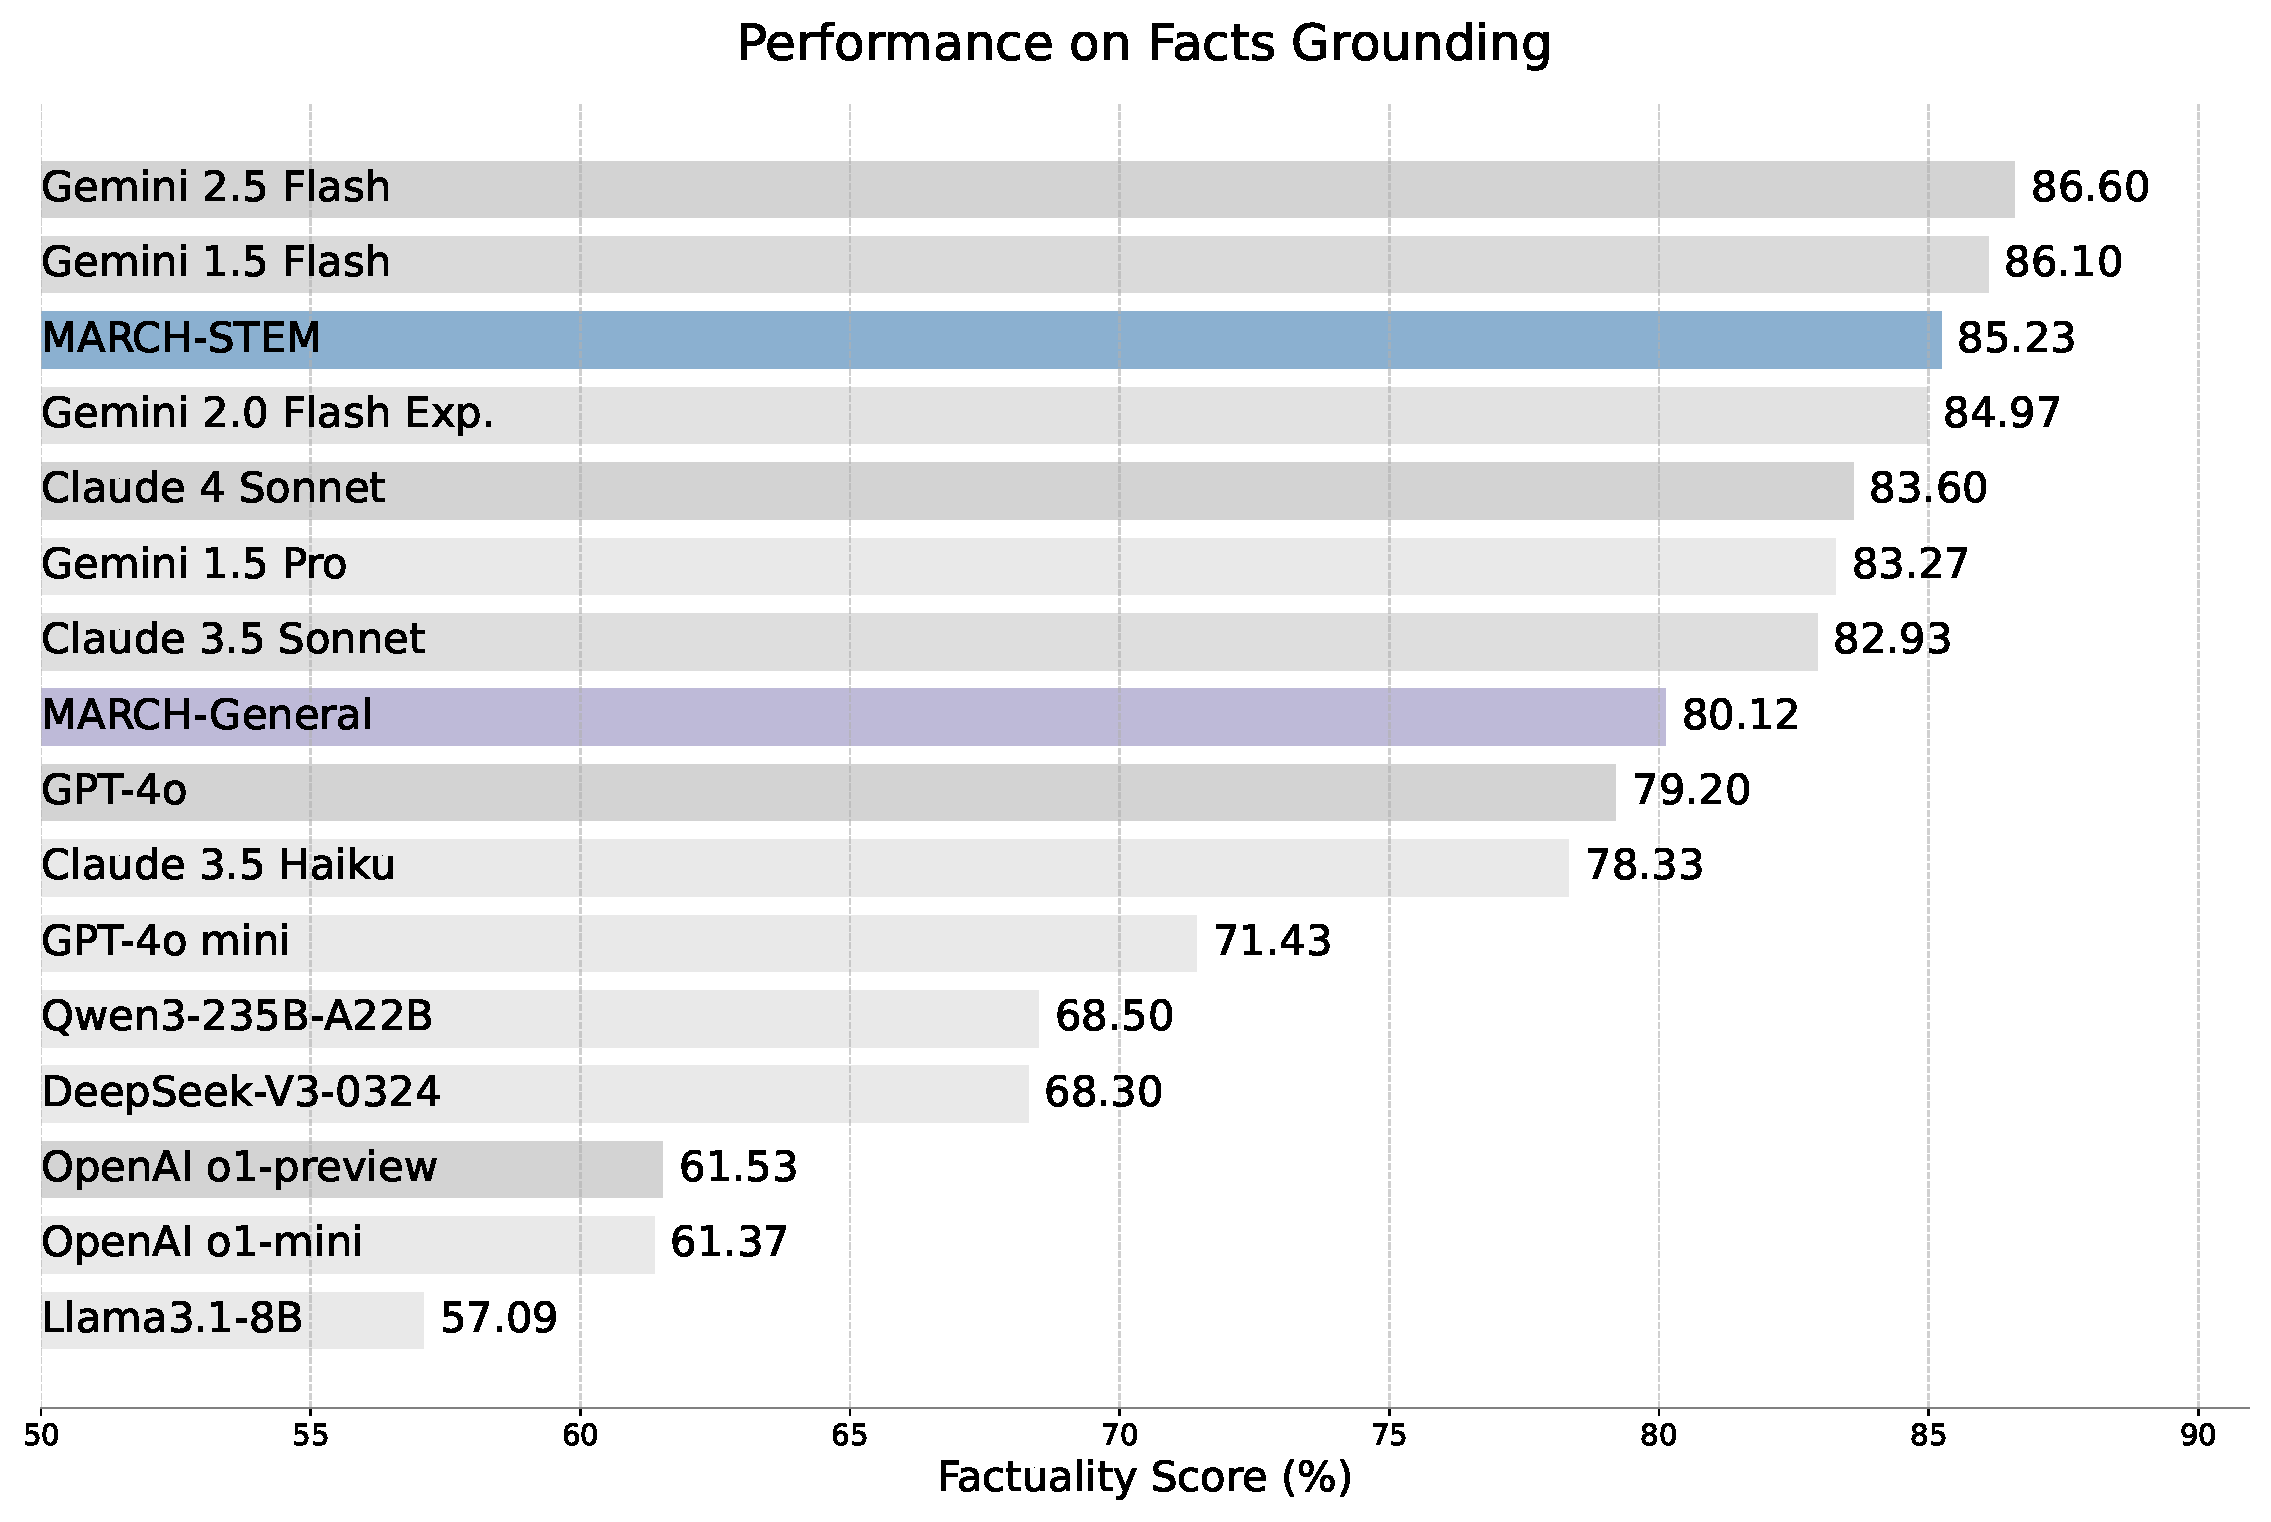
\includegraphics[width=.7\linewidth]{figures/facts_grounding.pdf}
    \caption{Comparison of performance on the Facts Grounding. MARCH (highlighted in blue and purple) demonstrates competitive performance against a range of leading open and proprietary models.}
    \label{fig:main_res_fg}
\end{figure}
\begin{table*}[!h]
\centering
\caption{Accuracy (\%) on ContextualJudgeBench. Baseline results are cited from~\citet{xu2025does}.}
\resizebox{\textwidth}{!}{% 使表格适应文本宽度
\begin{tabular}{l|ccccccccc}
\toprule
 \multirow{2}{*}{Model}  & {Refusal} & {Refusal} & {Faithfulness} & {Faithfulness} & {Completeness} & {Completeness} & {Conciseness} & {Conciseness} & \multirow{2}{*}{{Avg.}} \\
 & {(Ans.)} & {(Unans.)} & {(QA)} & {(Summ.)} & {(QA)} & {(Summ.)} & {(QA)} & {(Summ.)} & \\
\midrule
\rowcolor{mygray} \multicolumn{10}{c}{\textit{Small Judge Model}} \\
Glider-3.8B~\citep{deshpande2024glidergradingllminteractions} & 12.0 & 8.8 & 45.6 & 9.2 & 20.8 & 28.7 & 5.1 & 4.1 & 16.8 \\
Promtheus-2-7b~\citep{kim-etal-2024-prometheus} & 12.4 & 44.0 & 27.2 & 32.0 & 24.0 & 42.6 & 6.7 & 29.5 & 27.3 \\
Llama-3-OffsetBias-8B~\citep{park-etal-2024-offsetbias} & 64.8 & 11.2 & 34.0 & 26.4 & 33.2 & 21.1 & 46.3 & 23.0 & 32.6 \\
Skywork-8B~\citep{liu2024skyworkrewardbagtricksreward} & 60.8 & 12.0 & 38.8 & 31.6 & 38.4 & 26.7 & 29.4 & 21.3 & 32.4 \\
Alta-Selene-8B~\citep{alexandru2025atlaseleneminigeneral} & 74.4 & 26.4 & 40.8 & 32.8 & 32.4 & 34.7 & 23.1 & 32.0 & 37.1 \\
SFRJudge-8B~\citep{wang2025directjudgementpreferenceoptimization} & 70.8 & 22.0 & 40.4 & 38.8 & 40.4 & 43.4 & 27.5 & 31.1 & {39.3} \\
SFRJudge-12B~\citep{wang2025directjudgementpreferenceoptimization} & 68.4 & 28.4 & 45.2 & 43.6 & 28.0 & 51.0 & 16.1 & 29.5 & 38.8 \\
\midrule
\rowcolor{mygray} \multicolumn{10}{c}{\textit{ Large Judge Model}} \\
Promtheus-2-8x7b~\citep{kim-etal-2024-prometheus} & 22.0 & 29.6 & 22.4 & 29.6 & 20.4 & 39.8 & 10.2 & 18.4 & 24.1 \\
Skywork-70B~\citep{liu2024skyworkrewardbagtricksreward} & 82.4 & 11.2 & 48.0 & 47.6 & 36.8 & 41.4 & 21.6 & 27.9 & 39.6 \\
ST-Eval-70B~\cite{wang2024selftaughtevaluators} & 50.0 & 42.0 & 51.2 & 45.6 & 40.8 & 39.4 & 36.1 & 29.9 & 41.9 \\
SFRJudge-70B~\citep{wang2025directjudgementpreferenceoptimization} & 87.6 & 32.4 & 60.8 & \bb{54.8} & 40.8 & 53.4 & \bb{44.7} & 36.1 & {51.4} \\
\midrule
\rowcolor{mygray} \multicolumn{10}{c}{\textit{Instruct + Reasoning Model}}   \\
% & Llama-3.1-8B & 28.0 & 43.2 & 34.8 & 34.8 & 23.2 & 41.0 & 11.4 & 21.3 & 29.7 \\
Llama-3.1-70B~\citep{touvron2023llamaopenefficientfoundation} & 59.6 & 48.0 & 58.0 & 48.4 & 38.0 & 51.8 & 15.7 & 27.5 & 43.4 \\
Llama-3.3-70B~\citep{touvron2023llamaopenefficientfoundation} & 71.6 & 42.4 & 68.0 & 48.4 & 42.0 & 51.8 & 20.8 & 30.7 & 47.0 \\
R1Distill-Llama-3.3-70B~\citep{deepseekai2025deepseekr1incentivizingreasoningcapability} & \bb{89.6} & 50.4 & \rr{74.0} & 48.4 & 42.4 & 57.4 & 19.2 & 29.5 & 51.4 \\
GPT-4o-mini & 71.2 & 22.8 & 45.6 & 42.4 & 33.2 & 54.2 & 11.8 & 29.5 & 38.8 \\
GPT-4o & 64.0 & 52.0 & 68.0 & 50.8 & 39.6 & 56.2 & 12.9 & 22.5 & 45.8 \\
DeepSeek-R1~\citep{deepseekai2025deepseekr1incentivizingreasoningcapability} & \rr{92.0} & 52.0 & \bb{72.0} & 50.4 & 41.2 & 60.6 & 20.4 & 26.2 & \bb{51.9} \\
\midrule
\rowcolor{mygray} \multicolumn{10}{c}{\textit{OURS}}   \\
Llama-3.1-8B & 28.0 & 43.2 & 34.8 & 34.8 & 23.2 & 41.0 & 11.4 & 21.3 & 29.7 \\
% (General, w/ Solver)  & 35.8 & 61.6 & 54.4 & \bb{54.8} & 45.0 & 64.0 & 41.6 & 46.6 & {50.5} \\
\rowcolor{blue!5}\textbf{MARCH-General}       & 37.2 & 57.8 & 52.6 & \bb{54.8} & \rr{48.0} & \bb{63.9} & \rr{48.1} & \rr{50.1} & {51.6} \\
\rowcolor{blue!5}$\Delta$ & \textcolor{ggg}{$\uparrow9.2$} & \textcolor{ggg}{$\uparrow14.6$} & \textcolor{ggg}{$\uparrow17.8$} & \textcolor{ggg}{$\uparrow20.0$} & \textcolor{ggg}{$\uparrow24.8$} & \textcolor{ggg}{$\uparrow22.9$} & \textcolor{ggg}{$\uparrow36.7$} & \textcolor{ggg}{$\uparrow28.8$} & \textcolor{ggg}{$\uparrow21.9$} \\ 
% (STEM, w/ Solver)      & 37.4 & \bb{61.9} & 51.2 & 53.5 & \bb{46.4} & 62.0 & 43.8 & 46.4 & {50.3} \\
% Llama-3.1-8B & 28.0 & 43.2 & 34.8 & 34.8 & 23.2 & 41.0 & 11.4 & 21.3 & 29.7 \\
\rowcolor{blue!5}\textbf{MARCH-STEM}      & 38.1 & \rr{64.0} & 53.6 & \rr{58.0} & 44.9 & \rr{65.5} & \bb{44.7} & \bb{49.5} & \rr{52.3} \\
\rowcolor{blue!5}$\Delta$ & \textcolor{ggg}{$\uparrow10.1$} & \textcolor{ggg}{$\uparrow20.8$} & \textcolor{ggg}{$\uparrow18.8$} & \textcolor{ggg}{$\uparrow23.2$} & \textcolor{ggg}{$\uparrow21.7$} & \textcolor{ggg}{$\uparrow24.5$} & \textcolor{ggg}{$\uparrow33.3$} & \textcolor{ggg}{$\uparrow28.2$} & \textcolor{ggg}{$\uparrow22.6$} \\ 
\bottomrule
\end{tabular}
} \label{tab:comp_main_res_cjb}
\end{table*}
\paragraph{Results on ContextualJudgeBench.} Table~\ref{tab:comp_main_res_cjb} reports results on ContextualJudgeBench, which evaluates multiple dimensions of judge behavior, including refusal, faithfulness, completeness, and conciseness. Starting from Llama3.1-8B, our framework again yields large gains across all eight dimensions under both training regimes. Specifically, the policy trained on General QA data (\textit{MARCH-General}) improves the average accuracy from 29.7 to 51.6 ({+21.9}), while the policy trained on STEM data (\textit{MARCH-STEM}) reaches 52.3 ({+22.6}). The improvements are particularly pronounced on faithfulness and completeness (both QA and summarization), where accurate document-grounded judgment is most critical. Based on an 8B LLM, our policies surprisingly reach or surpass the performance of many much larger judge models, and approach the best specialized judge models on several dimensions. Table~\ref{tab:comp_main_res_cjb} indicates that MARCH not only improves binary hallucination detection but also equips LLM with a more nuanced ability to assess answer quality along multiple axes, such as whether key information is covered and whether responses remain concise and well-calibrated in context.

\subsection{Experiments on Multi-Hop QA}
Intuitively, the capacity for precise factual extraction and verification reasonably serves as the fundamental bedrock for complex reasoning, as Question Answering tasks usually require a model to sequentially bridge information across disparate documents. 
% As a result, any hallucination of a key entity or numerical value in the early hops will inevitably lead to a cascaded failure in the final synthesis. 
In this section, we empirically find that the improved factual grounding brought by MARCH can directly translate into better performance on reasoning-intensive downstream tasks.

\paragraph{Evaluation Benchmarks.} Following~\citet{xu2025collab,trivedi2023interleaving,shao2023enhancing}, we evaluate the performance of our MARCH on three popular multi-hop QA datasets, including HotpotQA~\citep{yang2018hotpotqa}, 2WikiMultiHopQA~\citep{ho2020constructing} and MuSiQue~\citep{trivedi2022musique}. More details about datasets are provided in Appendix~\ref{app:eval-details-qa}.

\paragraph{Evaluation Protocol and Metrics.}
Following~\citet{xu2025collab,shao2023enhancing,trivedi2023interleaving}, we sample the first 500 examples from the development set of each dataset as our evaluation subset to reduce the evaluation overhead while maintaining statistical reliability. For each question, the model receives the query and its associated context passages and produces a corresponding answer. We report accuracy (\%) with respect to the GT reference answers judged by a Qwen3-235B-A22B, using the official evaluation scripts when available. We also draw {eight} independent generations for each test query and then adopt a majority voting to decide the final verdict.

\begin{table}[!h]
\centering
\caption{Comparison of MARCH-Best against RAG baselines. {MARCH-Best} denotes our best-performing model. \underline{Underline} indicates the best performance among 8B-class models, and \textbf{Bold} indicates the best overall performance. Baseline results are cited from~\citet{xu2025collab}.}
\label{tab:sota_comparison}
\resizebox{0.7\textwidth}{!}{
\begin{tabular}{l c c c c}
\toprule
{Method} & {Backbone} & {HotpotQA} & {MuSiQue} & {2WikiMQA} \\
\midrule
\rowcolor{mygray} \multicolumn{5}{c}{\textit{Advanced RAG Frameworks with Proprietary Models}} \\
CoT \citep{wei2022chain} & GPT-4o & 56.2 & 26.8 & 58.4 \\
RAG-Standard \citep{lewis2020retrieval} & GPT-4o & 64.0 & 29.8 & 57.8 \\
IRCoT \citep{trivedi2022musique} & GPT-4o & 66.4 & \textbf{44.2} & \textbf{78.0} \\
Iter-RetGen \citep{shao2023enhancing} & GPT-4o & 62.6 & 42.0 & 71.4 \\
RAG-Star \citep{jiang2024ragstarenhancingdeliberativereasoning} & GPT-4o & 57.0 & 40.0 & 63.0 \\
RQ-RAG \citep{chan2024rqraglearningrefinequeries} & GPT-4o & 62.0 & 31.6 & 60.2 \\
\midrule
\rowcolor{mygray} \multicolumn{5}{c}{\textit{Specialized RAG Micro-tuning (White-box 7B/8B)}} \\
Baseline & Llama3.1-8B & 35.0  & 5.6 & 17.4 \\
GenGround \citep{shi2024generate} & 7B-class & 47.2 & 20.2 & 45.6 \\
RAFT \citep{dong2023raftrewardrankedfinetuning} & Llama3.1-8B & 51.2 & 22.0 & 44.6 \\
IRCoT \citep{trivedi2022musique} & Llama3.1-8B & 64.0 & 29.2 & 56.8 \\
\midrule
\rowcolor{blue!5} {MARCH (10-Shots)} & {Llama3.1-8B} & \underline{\textbf{{73.6}}} & \underline{40.8} & {69.4} \\
\rowcolor{blue!5} {MARCH (CoT)} & {Llama3.1-8B} & {{70.6}} & {36.2} & \underline{}{70.6} \\
\bottomrule
\end{tabular}
}
\end{table}

\paragraph{Comparison with Existing Baselines.}
Table~\ref{tab:sota_comparison} compares MARCH-Best, which incorporates joint optimization of both the {Solver} and the {Checker} alongside CoT prompting, with various specialized RAG methods and proprietary models. Within the 8B-parameter scale, MARCH achieves higher accuracy on the HotpotQA and MuSiQue benchmarks compared to methods such as RAFT~\citep{dong2023raftrewardrankedfinetuning} and GenGround~\citep{shi2024generate}. Notably, on the HotpotQA benchmark, which contains a high density of noisy documents, MARCH reaches an accuracy of 71.2\%, exceeding the reported results of standard GPT-4o RAG (64.0\%) and the IRCoT~\citep{trivedi2023interleaving} framework using GPT-4o (66.4\%). 
% While MARCH shows a narrower margin on MuSiQue and 2WikiMQA when compared to complex multi-step retrieval frameworks, MARCH remains competitive among single-model open-source baselines. 
Table~\ref{tab:sota_comparison} suggests that MARCH can effectively enhance the factual reliability of smaller models in multi-hop reasoning scenarios, leading to performance that is comparable to and even higher than much larger proprietary models.

\subsection{Ablation Study and Further Investigation}
\paragraph{Performance Analysis of Joint Optimization.} Table~\ref{tab:res_main_QA} illustrates that the joint optimization of the {Solver} and the {Checker} consistently achieves the highest accuracy across all training strategies in both STEM and General benchmarks. A key observation is that while the Solver-only update provides a base improvement, the inclusion of the {Checker} significantly amplifies the model's reasoning capabilities, particularly in complex scenarios. Specifically, in the \textit{Few-Shot} setting for STEM, the joint model achieves a remarkable absolute gain of 11.6\% over the {Solver-only} version. These results suggest that the {Checker}'s auditing signal is crucial for leveraging the full potential of advanced prompting techniques like \textit{few-shot} and \textit{CoT}, as it effectively mitigates factual drift and ensures logical consistency throughout multi-hop reasoning trajectories. In summary, Table~\ref{tab:res_main_QA} suggests that by internalizing a claim-level auditing logic, MARCH significantly amplifies the efficacy of in-context learning and multi-step reasoning, ensuring that increased model capacity translates into verifiable factual accuracy rather than hallucinated complexity.

\paragraph{Does our method conflict with other boosting methods?}
As demonstrated in Table~\ref{tab:res_main_QA}, MARCH is highly orthogonal and can be seamlessly integrated with existing performance-boosting techniques, including RLHF, Few-Shot prompting, and CoT reasoning. When applied to the Llama3.1-8B-Instruct baseline, our method consistently achieves significant performance gains across all benchmarks. For instance, combining MARCH with CoT reasoning further elevates the average accuracy on STEM tasks from 50.93\% to 59.13\%, and on General tasks from 51.00\% to 57.80\%. Similarly, notable improvements are observed when MARCH is integrated with Few-Shot (10-Shots) configurations, reaching an average of 61.27\% on STEM. Table~\ref{tab:res_main_QA} indicates that MARCH does not conflict with traditional scaling or prompting methods; rather, it provides a complementary layer of factual rigor through its asymmetric self-play mechanism, leading to a cumulative enhancement in multi-hop question-answering capabilities. We provide the implementation details in Appendix~\ref{app:baselines}.

% \begin{figure}[!t]
%     \centering
%     \includegraphics[width=0.7\linewidth]{figures/performance_gain.pdf}
% \caption{Averaged results on MuSuQueQA, 2WikiMultiHopQA and HotpotQA benchmarks across STEM (a) and General (b) training datasets based on Llama3.1-8B-Instruct. Comprehensive results are in Table~\ref{tab:res_main_QA}.}
%     \label{fig:avg_qa_performance_gain}
% \end{figure}
\begin{table*}[!t]
\centering
\caption{Main results on Multi-Hop Question Answering benchmarks across two training datasets based on Llama3.1-8B-Instruct. We report the accuracy rate (\%) by comparing the model output with the corresponding ground-truth label. We produce baseline results on our own environment.}
\resizebox{0.99\textwidth}{!}{
\begin{tabular}{ccc|cccc|cccc}
\toprule
\multicolumn{3}{c|}{Training Dataset} & \multicolumn{4}{c|}{STEM} & \multicolumn{4}{c}{General} \\
Method & Solver & Checker & MuSiQue & 2Wiki & Hotpot & Average & MuSiQue & 2Wiki & Hotpot & Average \\ \midrule
\rowcolor{mygray} \multicolumn{11}{c}{\textit{Compare with Instruct Baseline}}   \\
\multicolumn{3}{c|}{Baseline} & 5.60 & 17.40 & 35.00 & 19.33 & 5.60 & 17.40 & 35.00 & 19.33 \\
\multirow{2}{*}{\textbf{+MARCH}} & \ding{52} & - &
12.80\textsuperscript{\scriptsize\textcolor{ggg}{$\uparrow 7.20$}} &
25.40\textsuperscript{\scriptsize\textcolor{ggg}{$\uparrow 8.00$}} &
49.40\textsuperscript{\scriptsize\textcolor{ggg}{$\uparrow 14.40$}} &
29.20\textsuperscript{\scriptsize\textcolor{ggg}{$\uparrow 9.87$}} &
12.20\textsuperscript{\scriptsize\textcolor{ggg}{$\uparrow 6.60$}} &
27.80\textsuperscript{\scriptsize\textcolor{ggg}{$\uparrow 10.40$}} &
54.80\textsuperscript{\scriptsize\textcolor{ggg}{$\uparrow 19.80$}} &
31.60\textsuperscript{\scriptsize\textcolor{ggg}{$\uparrow 12.27$}} \\
& \ding{52} & \ding{52} &
16.60\textsuperscript{\scriptsize\textcolor{ggg}{$\uparrow 3.80$}} &
35.40\textsuperscript{\scriptsize\textcolor{ggg}{$\uparrow 10.00$}} &
55.20\textsuperscript{\scriptsize\textcolor{ggg}{$\uparrow 5.80$}} &
35.73\textsuperscript{\scriptsize\textcolor{ggg}{$\uparrow 6.53$}} &
18.40\textsuperscript{\scriptsize\textcolor{ggg}{$\uparrow 6.20$}} &
38.60\textsuperscript{\scriptsize\textcolor{ggg}{$\uparrow 10.80$}} &
56.40\textsuperscript{\scriptsize\textcolor{ggg}{$\uparrow 1.60$}} &
37.80\textsuperscript{\scriptsize\textcolor{ggg}{$\uparrow 6.20$}} \\ \midrule

\rowcolor{mygray} \multicolumn{11}{c}{\textit{Compare with RLHF Baseline}}   \\
\multicolumn{3}{c|}{RLHF} & 24.20 & 49.60 & 60.40 & 44.73 & 24.20 & 56.40 & 65.40 & 48.67 \\
\multirow{2}{*}{\textbf{+MARCH}} & \ding{52} & - &
29.00\textsuperscript{\scriptsize\textcolor{ggg}{$\uparrow 4.80$}} &
49.60\textsuperscript{\scriptsize\textcolor{ggg}{$\uparrow 0.00$}} &
66.40\textsuperscript{\scriptsize\textcolor{ggg}{$\uparrow 6.00$}} &
48.33\textsuperscript{\scriptsize\textcolor{ggg}{$\uparrow 3.60$}} &
30.80\textsuperscript{\scriptsize\textcolor{ggg}{$\uparrow 6.60$}} &
56.40\textsuperscript{\scriptsize\textcolor{ggg}{$\uparrow 0.00$}} &
67.80\textsuperscript{\scriptsize\textcolor{ggg}{$\uparrow 2.40$}} &
51.67\textsuperscript{\scriptsize\textcolor{ggg}{$\uparrow 3.00$}} \\
& \ding{52} & \ding{52} &
29.40\textsuperscript{\scriptsize\textcolor{ggg}{$\uparrow 0.40$}} &
53.20\textsuperscript{\scriptsize\textcolor{ggg}{$\uparrow 3.60$}} &
66.20\textsuperscript{\scriptsize\textcolor{rrr}{$\downarrow 0.20$}} &
49.60\textsuperscript{\scriptsize\textcolor{ggg}{$\uparrow 1.27$}} &
30.80\textsuperscript{\scriptsize\textcolor{ggg}{$\uparrow 0.00$}} &
61.00\textsuperscript{\scriptsize\textcolor{ggg}{$\uparrow 4.60$}} &
69.00\textsuperscript{\scriptsize\textcolor{ggg}{$\uparrow 1.20$}} &
53.60\textsuperscript{\scriptsize\textcolor{ggg}{$\uparrow 1.93$}} \\ \midrule

\rowcolor{mygray} \multicolumn{11}{c}{\textit{Boosting with Few Shots (10-Shots)}}   \\
\multicolumn{3}{c|}{RLHF + Few Shots} & 29.20 & 55.20 & 61.20 & 48.53 & 29.40 & 55.20 & 60.60 & 48.43 \\
\multirow{2}{*}{\textbf{+MARCH}} & \ding{52} & - &
28.60\textsuperscript{\scriptsize\textcolor{rrr}{$\downarrow 0.60$}} &
58.60\textsuperscript{\scriptsize\textcolor{ggg}{$\uparrow 3.40$}} &
61.80\textsuperscript{\scriptsize\textcolor{ggg}{$\uparrow 0.60$}} &
49.67\textsuperscript{\scriptsize\textcolor{ggg}{$\uparrow 1.14$}} &
28.00\textsuperscript{\scriptsize\textcolor{rrr}{$\downarrow 1.40$}} &
57.20\textsuperscript{\scriptsize\textcolor{ggg}{$\uparrow 2.20$}} &
62.20\textsuperscript{\scriptsize\textcolor{ggg}{$\uparrow 1.60$}} &
49.13\textsuperscript{\scriptsize\textcolor{ggg}{$\uparrow 0.70$}} \\
& \ding{52} & \ding{52} &
40.80\textsuperscript{\scriptsize\textcolor{ggg}{$\uparrow 12.80$}} &
69.40\textsuperscript{\scriptsize\textcolor{ggg}{$\uparrow 10.80$}} &
73.60\textsuperscript{\scriptsize\textcolor{ggg}{$\uparrow 11.80$}} &
61.27\textsuperscript{\scriptsize\textcolor{ggg}{$\uparrow 10.60$}} &
37.20\textsuperscript{\scriptsize\textcolor{ggg}{$\uparrow 9.20$}} &
62.00\textsuperscript{\scriptsize\textcolor{ggg}{$\uparrow 4.80$}} &
64.00\textsuperscript{\scriptsize\textcolor{ggg}{$\uparrow 1.80$}} &
54.40\textsuperscript{\scriptsize\textcolor{ggg}{$\uparrow 5.27$}} \\ \midrule

\rowcolor{mygray} \multicolumn{11}{c}{\textit{Boosting with Chain-of-Thought (CoT)}}   \\
\multicolumn{3}{c|}{RLHF + CoT} & 29.40 & 59.00 & 64.40 & 50.93 &  31.60 & 58.60 & 62.80 & 51.00 \\
\multirow{2}{*}{\textbf{+MARCH}} & \ding{52} & - &
32.40\textsuperscript{\scriptsize\textcolor{ggg}{$\uparrow 3.00$}} &
60.60\textsuperscript{\scriptsize\textcolor{ggg}{$\uparrow 1.60$}} &
64.00\textsuperscript{\scriptsize\textcolor{rrr}{$\downarrow 0.40$}} &
52.33\textsuperscript{\scriptsize\textcolor{ggg}{$\uparrow 1.40$}} &
32.40\textsuperscript{\scriptsize\textcolor{ggg}{$\uparrow 0.80$}} &
62.00\textsuperscript{\scriptsize\textcolor{ggg}{$\uparrow 3.40$}} &
68.20\textsuperscript{\scriptsize\textcolor{ggg}{$\uparrow 5.40$}} &
54.20\textsuperscript{\scriptsize\textcolor{ggg}{$\uparrow 3.20$}} \\
& \ding{52} & \ding{52} &
36.20\textsuperscript{\scriptsize\textcolor{ggg}{$\uparrow 3.80$}} &
70.60\textsuperscript{\scriptsize\textcolor{ggg}{$\uparrow 10.00$}} &
70.60\textsuperscript{\scriptsize\textcolor{ggg}{$\uparrow 6.60$}} &
59.13\textsuperscript{\scriptsize\textcolor{ggg}{$\uparrow 6.80$}} &
38.40\textsuperscript{\scriptsize\textcolor{ggg}{$\uparrow 6.00$}} &
63.80\textsuperscript{\scriptsize\textcolor{ggg}{$\uparrow 1.80$}} &
71.20\textsuperscript{\scriptsize\textcolor{ggg}{$\uparrow 3.00$}} &
57.80\textsuperscript{\scriptsize\textcolor{ggg}{$\uparrow 3.60$}} \\ 
\bottomrule
\end{tabular}
}\label{tab:res_main_QA}
\end{table*}

\paragraph{Influence of Reward Formulations.} We evaluate two reward formulations: (i) {Error Rate Reward (ERR)}, a proportional penalty based on the ratio of incorrect claims, which is defined as $R_{\text{ERR}} = - \frac{N_{\text{err}}}{N_{\text{total}}}$, where $N_{\text{total}}$ is the total number of claims generated and $N_{\text{err}}$ is the number of claims identified as incorrect by the Checker. and (ii) {Zero-Tolerance Reward (ZTR)}, the binary constraint that enforces absolute consistency defined in \eqref{eq:ztr_reward}. As shown in Table~\ref{tab:all_rf_ablation}, while all RL-tuned configurations significantly outperform the vanilla baselines, ZTR consistently surpasses ERR (e.g., 61.25\% vs 55.46\% on Llama3.1 joint-training), suggesting that strict logical consistency is more effective for complex RAG tasks. Within the ZTR, the penalty-based scalar ($-1/0$) yields superior results compared to the incentive-based ($0/1$) setting, as the former provides a stronger corrective gradient to suppress hallucinations. 

\paragraph{Impact of Reward Scalars}
We further compare two scalar assignments within the ZTR framework: a penalty-based setting ($-1/0$) and an incentive-based setting ($0/1$). The second group in Table~\ref{tab:all_rf_ablation} on the STEM dataset show that the $-1/0$ configuration (59.06\%) significantly outperforms the $0/1$ setting (50.42\%). We hypothesize that because factual successes are relatively sparse during early training phases, the $0/1$ incentive fails to provide sufficient contrast between diverse erroneous paths. In contrast, the $-1/0$ setting establishes factual accuracy as the default expectation, providing a robust corrective gradient that effectively suppresses hallucinations.


\paragraph{Performance on Different Model Family.} As shown in the last group in Table~\ref{tab:all_rf_ablation}, the MARCH framework exhibits robust generalizability across different model families, with Qwen3-8B reflecting the same performance trajectory observed in Llama-based experiments. Specifically, MARCH elevates Qwen3-8B to average accuracies of 67.90\% and 68.11\% under General and STEM settings, respectively, marking a significant absolute gain of over 11\% compared to its vanilla baseline (56.84\%) and demonstrating that the dual-trajectory optimization mechanism is model-agnostic and consistently internalizes superior evidentiary grounding across diverse architectures.

\begin{table*}[t]
\centering
\caption{Ablation study on reward functions, scalars and base LLMs.  We compare Error Rate Reward (ERR) and Zero-Tolerance Reward (ZTR) under different training configurations.}
\label{tab:all_rf_ablation}
\resizebox{\textwidth}{!}{
\begin{tabular}{c|c|cc|cccc|ccc|c}
\toprule
 Reward & Reward & \multirow{2}{*}{Solver} & \multirow{2}{*}{Checker} & \multicolumn{3}{c}{RAGTruth} & \multirow{2}{*}{Facts Grounding} & \multirow{2}{*}{MuSiQue} & \multirow{2}{*}{2Wiki} & \multirow{2}{*}{Hotpot} & \multirow{2}{*}{Average} \\ 
Function & Scalar &  &  & Summary & Data2Txt & QA &  &  &  &  &  \\ \midrule
\multicolumn{4}{c|}{Llama3.1-8B Baseline} & 71.33 & 28.67 & 63.31 & 57.09 & 5.60 & 17.40 & 35.00 & 39.77 \\ 
\rowcolor{mygray} \multicolumn{12}{c}{\textit{Ablation Study on Reward Function, General Training Dataset}} \\
ERR & - & \ding{52} & - & 80.00 & 49.33 & 74.82 & 71.98 & 10.60 & 24.80 & 52.00 & 51.93 \\ 
ZTR & -1/0 & \ding{52} & - & 88.67 & 66.67 & 82.73 & 80.12 & 12.20 & 27.80 & 54.80 & 59.00 \\ \midrule
ERR & - & \ding{52} & \ding{52} & 87.33 & 62.67 & 76.26 & 76.98 & 9.80 & 25.60 & 49.60 & 55.46 \\
ZTR & -1/0 & \ding{52} & \ding{52} & 89.33 & 66.67 & 82.73 & 76.63 & 18.40 & 38.60 & 56.40 & 61.25 \\
\rowcolor{mygray} \multicolumn{12}{c}{\textit{Ablation Study on Reward Scalar, STEM Training Dataset}} \\
\multirow{4}{*}{ZTR}  & 0/1 & \ding{52} & - & 78.00 & 42.00 & 75.54 & 68.84 & 7.4 & 25.00 & 48.85 & 49.38 \\ 
& -1/0 & \ding{52} & - & 80.58 & 51.33 & 80.50 & 77.09 & 12.80 & 25.40 & 49.40 & 53.87 \\ \cmidrule{2-12}
 & 0/1 & \ding{52} & \ding{52} & 74.67 & 54.67 & 79.14 & 69.65 & 6.8 & 25.20 & 42.80 & 50.42 \\
 & -1/0 & \ding{52} & \ding{52} & 83.33 & 58.67 & 82.73 & 81.51 & 16.60 & 35.40 & 55.20 &  59.06\\ \midrule
\rowcolor{mygray} \multicolumn{12}{c}{\textit{Ablation Study on Different Base LLM}} \\
 \multicolumn{4}{c|}{Qwen3-8B Baseline} & 54.00 & 28.50 & 61.15 & 52.41 & 48.00 & 72.40 & 81.50 & 56.84 \\
\multirow{1}{*}{General} & \multirow{1}{*}{ZTR}& \ding{52} & \ding{52} & 72.00 & 47.67 & 75.90 & 64.45 & 53.20 & 76.90 & 85.20 & 67.90 \\
\multirow{1}{*}{STEM} & \multirow{1}{*}{ZTR}& \ding{52} & \ding{52} & 74.67 & 48.00 & 74.10 & 64.19 & 53.60 & 76.20 & 86.00 & 68.11 \\
 \bottomrule
\end{tabular}
}
\end{table*}

\subsection{Additional Analysis}
We analyze the potential reward hacking in MARCH and provide a primary solution (Appendix~\ref{app:question_number_varying}). We visualize the PPO training dynamics and analyze the time consumption (Appendix~\ref{app:training_dy}), where we find the consistently increasing rewards and acceptable trade-off between training consumption and improved performance. We present cases to show outputs of each agent during one training step (Appendix~\ref{app:case_study} ).

\section{Related Work}
\paragraph{Hallucinations and Fact-Check in RAG.}
While RAG reduces fabrications by anchoring responses in external context \citep{lewis2020retrieval}, LLMs remain susceptible to context-conflicting hallucinations \citep{shuster2021retrievalaugmentationreduceshallucination}. Current mitigation efforts largely revolve around outcome-level supervision~\citep{shi2023replugretrievalaugmentedblackboxlanguage,gekhman2024doesfinetuningllmsnew,yu2024chainofnoteenhancingrobustnessretrievalaugmented,asai2023selfraglearningretrievegenerate}, post-hoc reasoning refinements and utilizing external verifiers to filter outputs during inference \citep{dhuliawala2023chainofverificationreduceshallucinationlarge,madaan2023selfrefineiterativerefinementselffeedback,min-etal-2023-factscore,rashkin2023measuring,gao-etal-2023-rarr,tang2024minicheck}. However, these methods often treat LLM as a black box and fail to internalize factual constraints within the training objective itself. Moving beyond, we propose a framework where the model learns to prioritize factual adherence by minimizing logical discrepancies identified through an internal audit.

\paragraph{Multi-Agent Systems for LLMs.}
Multi-agent systems have emerged as a robust paradigm for enhancing LLM performance through collaborative or adversarial interactions \citep{du2023improvingfactualityreasoninglanguage,li2023camel}, which typically assign distinct personas to one / multiple model instances to facilitate code generation~\citep{huang2023agentcoder,islam2024mapcoder}, complex reasoning~\citep{li2023camel,he2023lego,talebirad2023multi}, decision-making~\citep{shinn2023reflexion,yu2024fincon}, recommendation~\citep{wang2024macrec}, and debate-driven consensus \citep{du2023improvingfactualityreasoninglanguage,liang2024encouraging}. While effective at inference time, most existing architectures treat agents as separate entities, often overlooking the potential for joint policy optimization across different functional roles. In addition, previous work shows that multi-agent system sometimes amplifies the hallucination of LLMs~\citep{hong2023metagpt}. Our framework differs by instantiating functionally distinct roles within a single shared policy. By structurally enforcing an information barrier between agents, we facilitate the co-evolution of generative and evaluative capabilities within a unified training loop, ensuring that the model’s internal verification logic directly informs its generative precision.

\section{Conclusion}
\vspace{-2mm}
%This paper presented MARCH to mitigate hallucinations in data-intensive RAG tasks. By transforming a shared policy into a coordinated hierarchy of the Solver, the {Proposer}, and the {Checker}, MARCH enables LLMs to concurrently evolve reasoning synthesis and independent grounding capabilities. Our results across various benchmarks demonstrate that the Zero-Tolerance Reward and dual-trajectory PPO effectively internalize a self-contained verification loop, yielding significant performance gains over strong baselines. MARCH's generalization across different model families underscores the potential as a scalable solution for high-fidelity information synthesis in complex knowledge domains.

In this paper, we introduced MARCH, a multi-agent framework designed to mitigate hallucinations in data-intensive RAG tasks. By reconfiguring a shared policy into a coordinated hierarchy comprising a Solver, a Proposer, and a Checker, MARCH enables LLMs to simultaneously refine their synthesis reasoning and independent grounding capabilities. Our experiments demonstrate that the combination of a Zero-Tolerance Reward mechanism and dual-trajectory PPO effectively internalizes a self-contained verification loop, consistently outperforming strong baselines. The robust generalization of MARCH across diverse model families underscores its potential as a scalable, high-fidelity solution for information synthesis in complex knowledge domains. We believe this agentic co-evolution paradigm offers a promising pathway toward building inherently trustworthy and verifiable large language models.

\bibliography{iclr2026_conference}
\bibliographystyle{iclr2026_conference}

\appendix

\section{Methodology}
\subsection{System Prompt of the \textit{Solver} Agent}\label{app:answer_prompt}

\begin{tcolorbox}[
    enhanced,
    colback=promptpurple,          % 背景色：淡紫色
    colframe=bordergray,           % 边框颜色：深灰色
    boxrule=1pt,                   % 边框粗细
    sharp corners,                 % 图像中是直角或极微小圆角，此处用直角
    fontupper=\ttfamily,           % 模仿图片中的等宽字体(Typewriter)风格
    left=15pt,                     % 左内边距
    right=15pt,                    % 右内边距
    top=12pt,                      % 上内边距
    bottom=12pt                    % 下内边距
]
\begin{flushleft}
    \textbf{Instruction:} \\
    You must respond based strictly on the information in provided passages. 
    Do not incorporate any external knowledge or infer any details beyond what is given in the passages. \\
    \vspace{1em}
    
    \textbf{Passages $D$:} \\
    \{Document-1\} \\
    ... \\
    \{Document-K\} \\
    \vspace{1em}
    
    \textbf{Query $\mathbf{x}$:} \\
    \{User Query $\mathbf{x}$\} \\
    \vspace{1em}
    
    \textbf{Output:}
\end{flushleft}
\end{tcolorbox}

\subsection{System Prompt of the \textit{Proposer} Agent}\label{app:propose_qa}
\begin{tcolorbox}[
    enhanced,
    colback=promptgreen,           % 背景色：淡绿色
    colframe=bordergray,           % 边框颜色：深灰色
    boxrule=1pt,                   % 边框粗细
    sharp corners,                 % 图像中是直角或极微小圆角，此处用直角
    fontupper=\ttfamily,           % 模仿图片中的等宽字体(Typewriter)风格
    left=15pt,                     % 左内边距
    right=15pt,                    % 右内边距
    top=12pt,                      % 上内边距
    bottom=12pt                    % 下内边距
]
\begin{flushleft}
    \textbf{You are a data annotation expert.} Your task is to analyze a model's response to a user query. For every critical number found in the model's response, you must create a question where the answer is precisely and exactly that number. \\
    
    \textbf{Rule 1. Clarity and Specificity of Questions:} Each question must be clear, complete, and unambiguous. It must contain enough context from the response to ensure the number is the only possible correct answer. For example, if the model's response contains ``In 2025, 50 people will take the bar exam in Beijing,'' an effective question would be ``How many people will take the bar exam in the Beijing area in 2025?'', and the answer is 50. A bad example would be ``How many people will take the bar exam in 2025?''. This is ambiguous because it lacks the specific region ('Beijing area'). \\
    
    \textbf{Rule 2. Format of the Answer:} The answer must be a pure number, either an integer or a decimal. It must NOT include any other characters or formats, such as percentage signs (\%), 'k' to denote thousands (e.g., 10k), ranges (e.g., 10-20), or words (e.g., fifty). \\
    
    Please provide your output as an unordered list using the following format for each question-answer pair: \\
    \texttt{- Question: xxx [Answer: n]} \\
    \texttt{- Question: xxx [Answer: n]} \\
    
    Now, generate questions for the user query and model response below. Do not output any other content or explanations. \\
    
    \vspace{1em}
    
    \textbf{Model Response:} \\
    \{response $\mathbf{y}$\}
\end{flushleft}
\end{tcolorbox}

\subsection{System Prompt of the \textit{Checker} Agent}\label{app:check_qa}
\begin{tcolorbox}[
    enhanced,
    breakable,
    colback=promptblue,            % 背景色：淡蓝色
    colframe=bordergray,           % 边框颜色：深灰色
    boxrule=1pt,                   % 边框粗细
    sharp corners,                 % 图像中是直角或极微小圆角，此处用直角
    fontupper=\ttfamily,           % 模仿图片中的等宽字体(Typewriter)风格
    left=15pt,                     % 左内边距
    right=15pt,                    % 右内边距
    top=12pt,                      % 上内边距
    bottom=12pt                    % 下内边距
]
\begin{flushleft}
    \textbf{You are a data validation expert.} You will be given a set of reference materials and a list of user questions. Your task is to retrieve information from the reference materials to answer all questions. Before providing each answer, you must state the evidence for it. \\
    
    You must adhere strictly to the content of the reference materials and must not fabricate or infer any information that is not explicitly mentioned. If the relevant information cannot be found in the materials, you must state ``Cannot answer''. It is important to note that all answers are pure numbers. Therefore, your answer must also be a pure number and must not contain any other content, such as percentage signs (\%), 'k' to denote thousands, ranges, or numbers written as words. \\
    
    \textit{Here is an example:} \\
    \textbf{Reference Materials:} \\
    Document 1: ...in 2024, 50 people will take the bar exam in Beijing. \\
    Document 2: ...(omitted) \\
    
    \vspace{0.5em}
    - Question 1: How many people will take the bar exam in Beijing in 2024? \\
    - Question 2: How many people will take the bar exam in Beijing in 2025? \\
    
    \vspace{0.5em}
    \textbf{Example Response:} \\
    1. Evidence: Document 1 states that 50 people will take the bar exam in Beijing in 2024.\\
    \texttt{[Answer: 50]} \\
    2. Evidence: The materials do not contain information about the bar exam in Beijing for 2025, therefore I cannot answer. \\
    \texttt{[Answer: Cannot answer]} \\
    
    Now, based on the reference materials below, answer all the following questions. Strictly adhere to the example format provided. \\
    
    \vspace{1em}
    \textbf{Reference Materials:} \\
    \{docs $D$\} \\
    
    \textbf{Questions:} \\
    \{questions $\mathbf{q}^{\text{aux}}$\}
\end{flushleft}
\end{tcolorbox}

\section{Experiment}\label{app:exp}

\subsection{Training Details}\label{app:training_hp}
We give more detailed training hyper-parameters in the Table~\ref{tab:hyperparams}.

\begin{table}[!h]
\centering
\caption{Key hyperparameters for our RL training, derived from the execution script.}
\label{tab:hyperparams}
\resizebox{0.7\textwidth}{!}{%
\begin{tabular}{llc}
\toprule
\multirow{3}{*}{Data \& Model Configuration} & Max Prompt Length & 24,567 \\
& Max Response Length & 8,192 \\
& Filter Overlong Prompts & True \\
\midrule
\multirow{4}{*}{Optimizer \& Learning Rates} & Actor Learning Rate & \(1 \times 10^{-6}\) \\
& Critic Learning Rate & \(1 \times 10^{-5}\) \\
& Actor LR Warmup Steps & 5 \\
& Critic LR Warmup Steps & 10 \\
\midrule
\multirow{2}{*}{PPO Algorithm \& Rewards} & $\gamma$ & 0.998 \\
& KL Divergence Coefficient & \(1 \times 10^{-3}\) \\
\midrule
\multirow{2}{*}{Training Schedule} & Total Epochs & 1 \\
& Global Batch Size / Mini-batch Size & 32 \\
\midrule
\multirow{2}{*}{Rollout (Training)} & Inference Engine & \texttt{vLLM} \\
&  Temperature & 0.6 \\ \midrule
\multirow{6}{*}{Rollout (Evaluation)} & Inference Engine & \texttt{vLLM} \\
&  Temperature & 0.6 \\
&  Batch Size & 32/32 \\
&  Top-P & 0.95 \\
&  Top-K & 20 \\
&  Rollout Number & 8 \\
\bottomrule
\end{tabular}%
}
\end{table}
\subsection{Evaluation Details}

\subsubsection{Hallucination and Factual Grounding Benchmarks}\label{app:eval-details-fc}
\paragraph{RAGTruth and FaithBench} are public benchmarks for evaluating hallucinations in retrieval-augmented generation, which contain three task types: (i) QA, (ii) Data2Txt Writing, and (iii) Summarization, each with human-annotated hallucinations at the response level. For each example, the model is given a query and a set of retrieved passages, and asked to produce an answer, a data-to-text description, or a summary. 

\paragraph{Contextual JudgeBench} is a judge benchmark with 2,000 challenging response pairs across eight splits inspired by real-world contextual evaluation scenarios, which is built with a multi-pronged data construction pipeline that leverages both existing human annotations and model-based perturbations. The evaluation task requires a model to act as a judge, choosing the better of two provided responses (A and B) according to specific, context-dependent criteria.

\paragraph{Facts Grounding} is a large-scale factuality benchmark spanning five domains (e.g., medical, financial, legal, and others) and nine task types, including summarization, fact finding, comparison, and definition. Each instance consists of a query, a collection of documents, and a reference output with fine-grained factual annotations, providing a broad and challenging testbed for document-grounded evaluation. During test, we adopt the official \texttt{JSON} judgment prompt provided by~\citet{jacovi2025facts}.

\subsubsection{QA Benchmarks}\label{app:eval-details-qa}

\paragraph{HotpotQA.}
HotpotQA~\citep{yang2018hotpotqa} is a large-scale multi-hop QA dataset that requires reasoning over multiple Wikipedia passages to answer fact-based questions. Each question is paired with multiple supporting paragraphs and a short, factoid-style answer.

\paragraph{2WikiMultiHopQA.}
2WikiMultiHopQA~\citep{ho2020constructing} extends HotpotQA with questions that require reasoning across two different Wikipedia articles, emphasizing cross-document retrieval and multi-hop reasoning over disjoint evidence.

\paragraph{MuSiQue.}
MuSiQue~\citep{trivedi2022musique} is a challenging multi-hop QA dataset with questions that explicitly require reasoning across multiple sentences scattered across different documents, often involving compositional reasoning over several intermediate facts.


\subsection{Baseline Methods}
\label{app:baselines}

\paragraph{Baselines.}
The raw backbone model used in all settings, evaluated in a zero-shot manner with task-specific instructions but without additional reasoning or RL fine-tuning. 

\paragraph{+CoT.}
A prompting baseline where we encourage step-by-step reasoning by prepending chain-of-thought instructions (e.g., ``let's think step by step'') to the prompt. The model is still the same base LLM; only the decoding prompt is changed.

\paragraph{+Few-Shot.}
An in-context learning baseline where we augment the prompt with a small number of annotated QA examples (few-shot demonstrations) drawn from the training distribution, following standard practice in multi-hop QA and factuality evaluation.

\paragraph{+RLHF.}
A version of the base LLM further optimized with reinforcement learning from human feedback, using general-purpose reward models that favor helpful and harmless responses but are not specifically tuned for document-grounded factuality. We adopt Skywork-Reward-V2-Llama-3.1-8B~\citep{liu2025skyworkrewardv2scalingpreferencedata} as the reward model.

% \subsection{Analysis of Internal Performance Gains}\label{app:performance_gain}
%  Table~\ref{tab:res_main_QA} demonstrates that joint optimization of the \textit{Solver} and the \textit{Checker} outperforms both baseline configurations and the \textit{Solver}-only updates across most benchmarks. A key observation is the stability provided by the \textit{Checker} role in complex reasoning scenarios. Specifically, while a \textit{Solver}-only update can lead to performance regressions under 10-shot prompting (e.g., dropping from 29.20 to 28.60 on MuSiQue STEM), the joint update effectively reverses this trend, reaching 40.80, highlighting that the \textit{Checker} acts as a critical anchor by preventing factual drift when the model is tasked with extended prompts. Notably, the benefits of MARCH are most pronounced when integrated with advanced prompting strategies like Few-shot and CoT. The average STEM score improvement (Joint vs. the \textit{Solver}-only) increases from 1.27 points in the RLHF setting to 10.60 points in the Few-shot setting and 6.80 points in the CoT setting. In summary, Table~\ref{tab:res_main_QA} suggests that by internalizing a claim-level auditing logic, MARCH significantly amplifies the efficacy of in-context learning and multi-step reasoning, ensuring that increased model capacity translates into verifiable factual accuracy rather than hallucinated complexity.

% \paragraph{Will filtering out noise docs help better performance?}
% \subsection{Extended Ablation Analysis}\label{app:ablation_extended}
% In this section, we provide a comprehensive analysis of the reward mechanisms and model-specific performance gains reported in Table~\ref{tab:compact_ablation} and Table~\ref{tab:all_rf_ablation}.


% \paragraph{Influence of Reward Formulations.} We investigate two primary reward designs:
% \begin{itemize}
%     \item \textbf{Error Rate (ER):} Defined as $R_{ER} = - \frac{N_{err}}{N_{total}}$, where $N_{total}$ is the total number of claims generated and $N_{err}$ is the number of claims identified as incorrect by the Checker. This provides a granular, proportional feedback signal.
%     \item \textbf{Zero-Tolerance Reward (ZTR):} Defined as $R_{ZTR} = -1$ if $N_{err} > 0$, and $0$ otherwise. This enforces a rigorous binary constraint, treating any single factual error as a failure of the entire response.
% \end{itemize}
% Our results indicate that ZTR consistently outperforms ER across both Solver-only and Joint training configurations. For instance, in the joint training setting, ZTR improves the average accuracy from 55.46\% (ER) to 61.25\% (ZTR). This confirms that for RAG tasks requiring high factual precision, a strict "all-or-nothing" penalty is more effective at internalizing logical consistency than a proportional reduction.



% \paragraph{Generalizability Across Model Families}
% To verify the model-agnostic nature of MARCH, we extend our evaluation to the Qwen3-8B family. The performance trajectory of Qwen3 mirrors that of Llama3.1, showing consistent gains across all benchmarks. Specifically, MARCH elevates the Qwen3-8B baseline from 56.84\% to a maximum of 68.11\% average accuracy when trained on STEM data. The specific task-level breakdown (e.g., 74.67\% on RAGTruth Summary and 86.00\% on HotpotQA) demonstrates that the dual-trajectory optimization consistently enhances both reasoning synthesis and evidentiary precision regardless of the underlying model architecture.


\subsection{How Would Proposed Question Numbers Influence Performance?}\label{app:question_number_varying}
A potential reward hacking of the MARCH framework could be that the system may attempt to inflate its reward by reducing the number of proposed questions, adhering to a ``less said, less leaked'' strategy where fewer claims minimize the probability of being audited as a hallucination. As illustrated in Figure~\ref{fig:q_number_stem}, we indeed observe a gradual decline in the average number of proposed questions as training progresses across all configurations. Notably, the configuration involving joint updates of the {Solver + Checker} exhibits a more pronounced downward trend compared to the {Solver Only} baseline, suggesting that the zero-tolerance penalty on the Checker's trajectory imposes a stricter consistency bottleneck, further incentivizing the \textit{Proposer} to prune potentially risky claims.

However, we find that this quantitative shrinkage can be effectively mitigated through simple instructional constraints. By explicitly requiring the \textit{Proposer} to generate no fewer than $k$ questions within the prompt (e.g., $k=3$), the decline in question density is significantly arrested. As shown by the solid lines in Figure~\ref{fig:q_number_stem}, models with such constraints in the legend (solid lines marked with ``w/ constraint'') maintain a much more stable and higher volume of factual inquiries throughout the self-evolution process, which indicates that the MARCH framework remains robust when balanced with basic task-specific instructions, ensuring that the drive for factual accuracy does not come at the cost of informational density.

 \begin{figure}[!h]
    \centering
    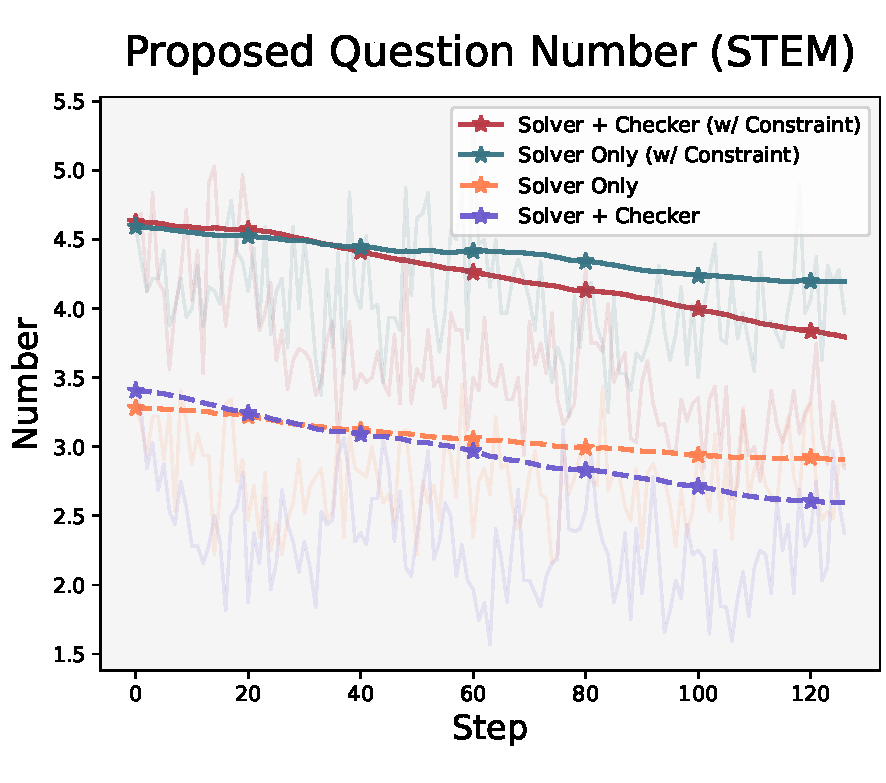
\includegraphics[width=0.5\linewidth]{figures/q_number_stem.pdf}
    \caption{Average number of proposed questions per step on the STEM training dataset. The dashed lines represent the MARCH framework without maintaining the question number, while the solid lines (w/ Constraint) indicate the results after incorporating instructional constraints to maintain informational density.}
    \label{fig:q_number_stem}
\end{figure}
\subsection{Visualization of Training Dynamics and Time Consuming}\label{app:training_dy}
To further investigate the practical efficiency of the MARCH framework, we analyze the training dynamics and computational overhead. Figures~\ref{fig:training_dyncs}(a)-(d) illustrate the stable convergence of accuracy and rewards across both General and STEM datasets, where the joint {Solver + Checker} update consistently outperforms the {Solver Only} configuration. Regarding training efficiency, Figure~\ref{fig:training_dyncs}(e) presents the cumulative time consumption on the General dataset (containing 9,000 samples), where we find that simultaneously updating both the \textit{Solver} and the \textit{Checker} trajectories in a single training step does not impose a prohibitive computational burden.

\begin{figure*}[!h]
    \centering
    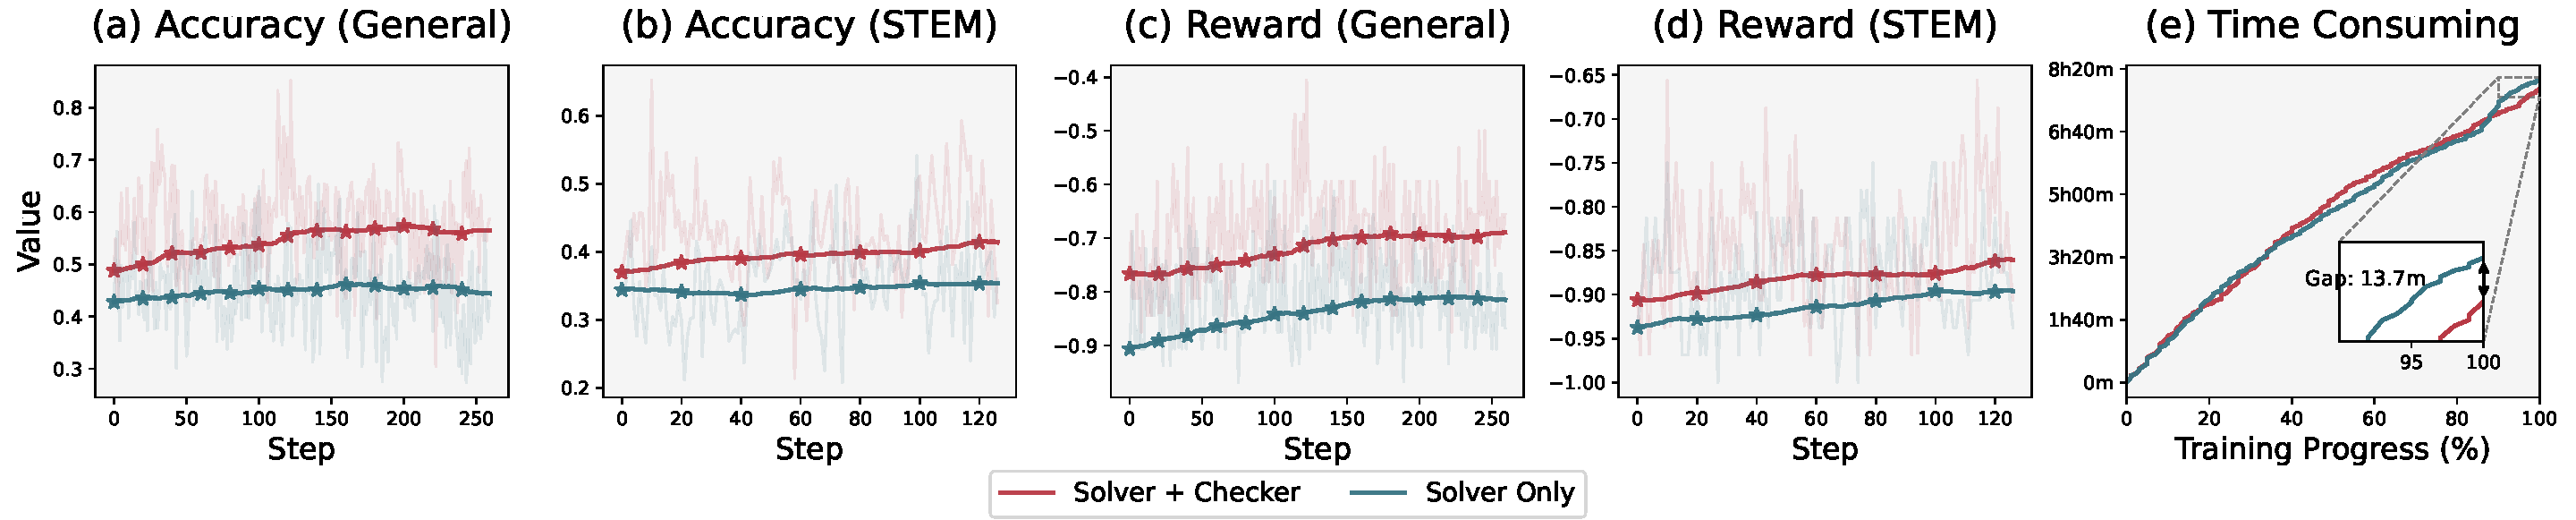
\includegraphics[width=1\linewidth]{figures/training_dyncs.pdf}
\caption{Visualization of training efficiency and dynamics. (a)-(d) illustrate the convergence of accuracy and rewards across general and STEM datasets. (e) Comparison of cumulative training time on the General dataset.}
    \label{fig:training_dyncs}
\end{figure*}

\section{Case Study}\label{app:case_study}
\subsection{Case 1}
\paragraph{Input $(\vx,\mD)$ of Agent Solver $\nu_\text{solve}$}

\begin{tcolorbox}[
    enhanced,
    breakable,
    colback=promptpurple,            % 背景色：淡蓝色
    colframe=bordergray,           % 边框颜色：深灰色
    boxrule=1pt,                   % 边框粗细
    sharp corners,                 % 图像中是直角或极微小圆角，此处用直角
    % fontupper=\ttfamily,           % 模仿图片中的等宽字体(Typewriter)风格
    % left=15pt,                     % 左内边距
    % right=15pt,                    % 右内边距
    % top=12pt,                      % 上内边距
    % bottom=12pt                    % 下内边距
]
\begin{flushleft}
You must respond based strictly on the information in the passages. Do not incorporate any external knowledge or infer any details beyond what is given in the passages.
\\
\vspace{1em}
\textbf{Passages:}\\
\textbf{Document-1}\\
TUDY OBJECTIVE: To describe sleep characteristics and rapid eye movement (REM) sleep behavior disorder in patients with Guadeloupean atypical parkinsonism (Gd-PSP)...(omit)...
% , a tauopathy resembling progressive supranuclear palsy that mainly affects the midbrain. It is possibly caused by the ingestion of sour sop (corossol), a tropical fruit containing acetogenins, which are mitochondrial poisons. DESIGN: Sleep interview, motor and cognitive tests, and overnight videopolysomnography. PATIENTS: Thirty-six age-, sex-, disease-duration- and disability-matched patients with Gd-PSP (n = 9), progressive supranuclear palsy (a tauopathy, n = 9), Parkinson disease (a synucleinopathy, n = 9) and controls (n = 9). SETTINGS: Tertiary-care academic hospital. RESULTS: REM sleep behavior disorder was found in 78\% patients with Gd-PSP (43\% of patients reported having this disorder several years before the onset of parkinsonism), 44\% of patients with idiopathic Parkinson disease, 33\% of patients with progressive supranuclear palsy, and no controls. The percentage of muscle activity during REM sleep was greater in patients with Gd-PSP than in controls (limb muscle activity, 8.3\%+\/-8.7\% vs 0.1\%+\/- 0.2\%; chin muscle activity, 24.3\%+\/- 23.7\% vs 0.7\%+\/-2.0\%) but similar to that of other patient groups. The latency and percentage of REM sleep were similar in patients with Gd-PSP, patients with Parkinson disease, and controls, whereas patients with progressive supranuclear palsy had delayed and shortened REM sleep. CONCLUSION: Although Gd-PSP is a tauopathy, most patients experience REM sleep behavior disorder. This suggests that the location of neuronal loss or dysfunction in the midbrain, rather than the protein comprising the histologic lesions (synuclein versus tau aggregation), is responsible for suppressing muscle atonia during REM sleep. 
Subjects with idiopathic REM sleep behavior disorder should avoid eating sour sop.
\\
\vspace{1em}
\textbf{Document-2}\\
We characterize the clinical features of Parkinson's syndrome on Guadeloupe and describe possible environmental causes...(omit)...
% Consecutive patients who were referred to the University Hospital at Pointe a Pitre with parkinsonism from September 1996 to May 2002 were included. All cases were examined in a standardized manner by a neurologist with a special interest in movement disorders and independently by 3 external movement disorders specialists, using standard operational clinical diagnostic criteria. The subjects were 265 patients with Parkinson's syndrome living on Guadeloupe, four fifths of whom had been referred by primary care physicians and one fifth by neurologists. The levodopa response was assessed after a minimum period of 1 month of continuous treatment. All patients had brain computed tomography or brain magnetic resonance imaging scans and detailed neuropsychological examinations. Of 265 patients, only 66 were classified as Parkinson's disease, whereas 58 fulfilled the National Institute of Neurological Disorders and Stroke (NINDS) and Society for Progressive Supranuclear Palsy (SPSP) criteria for progressive supranuclear palsy, 100 had unclassifiable parkinsonism, characterized by dopa-unresponsiveness, marked axial rigidity, relative symmetry of parkinsonian features, early dysarthria, and frontolimbic cognitive impairment. Within this group, early postural instability, dysarthria, a frontal behavior disorder, cortical or subcortical atrophy, pyramidal signs, axial rigidity, and family history of neurodegenerative disorders were associated with poorer prognosis. A very large number of unclassifiable cases of atypical parkinsonism that do not fulfill operational criteria for Parkinson's disease or other defined motor neurodegenerations has been observed on Guadeloupe. Most patients closely resemble descriptions of bodig from Guam. In both geographic isolates, an environmental cause has been discussed. Annonaceae fruits and herbal teas are consumed on both islands. These plants contain several neurotoxins, particularly acetogenins, which induce dopaminergic neuron loss in animals. Neuronal death involves cholinergic and dopaminergic cells of the substantia nigra and GABAergic neurons of the striatum, associated with microglial proliferation. 
The development of atypical parkinsonism in Guadeloupe and probably elsewhere, could result from synergistic toxicity, but acetogenins are probably the most potent neurotoxin, acting as mitochondrial complex I inhibitor.
\\
\vspace{1em}
\textbf{Document-3}\\
In Guadeloupe, there is an abnormally high frequency of atypical parkinsonism...(omit)...
% Only one-third of the patients that develop parkinsonian symptoms were reported to present the classical features of idiopathic Parkinson disease and one-third a syndrome resembling progressive supranuclear palsy (PSP). The others were unclassifiable, according to established criteria. We carried out a cross-sectional study of 160 parkinsonian patients to: (i) define more precisely the clinical phenotypes of the PSP-like syndrome and the parkinsonism that was considered unclassifiable in comparison with previously known disorders; (ii) define the neuropsychological and brain imaging features of these patients; (iii) evaluate to what extent a candidate aetiological factor, the mitochondrial complex I inhibitor annonacin contained in the fruit and leaves of the tropical plant Annona muricata (soursop) plays a role in the neurological syndrome. Neuropsychological tests and MRI were used to classify the patients into those with Parkinson's disease (31\%), Guadeloupean PSP-like syndrome (32\%), Guadeloupean parkinsonism-dementia complex (PDC, 31\%) and other parkinsonism-related disorders (6\%). Patients with a PSP-like syndrome developed levodopa-resistant parkinsonism, associated with early postural instability and supranuclear oculomotor dysfunction. They differed, however, from classical PSP patients by the frequency of tremor (>50\%), dysautonomia (50\%) and the occurrence of hallucinations (59\%). PDC patients had levodopa-resistant parkinsonism associated with frontosubcortical dementia, 52\% of these patients had hallucinations, but, importantly, none had oculomotor dysfunction. The pattern of neuropsychological deficits was similar in both subgroups. Cerebral atrophy was seen in the majority of the PSP-like and PDC patients, with enlargement of the third ventricle and marked T2-hypointensity in the basal ganglia, particularly the substantia nigra. Consumption of soursop was significantly greater in both PSP-like and PDC patients than in controls and Parkinson's disease patients. 
In conclusion, atypical Guadeloupean parkinsonism comprises two forms of parkinsonism and dementia that differ clinically by the presence of oculomotor signs, but have similar cognitive profiles and neuroimaging features, suggesting that they may constitute a single disease entity, and both were similarly exposed to annonaceous neurotoxins, notably annonacin.
\\
\vspace{1em}
\textbf{Document-4}\\
An unusually high frequency of atypical Parkinson syndrome has been delineated over the last 5 years in the French West Indies...(omit)... 
% Postural instability with early falls, prominent frontal lobe dysfunction and pseudo-bulbar palsy were common and three-quarters of the patients were L-dopa unresponsive. One-third of all patients seen had probable progressive supranuclear palsy (PSP). This new focus of atypical parkinsonism is reminiscent of the one described in Guam and may be linked to exposure to tropical plants containing mitochondrial complex I inhibitors (quinolines, acetogenins, rotenoids). Two hundred and twenty consecutive patients with Parkinson's syndrome seen by the neurology service at Pointe \u00e0 Pitre, Guadeloupe University Hospital were studied. Currently accepted operational clinical criteria for Parkinson's syndromes were applied. The pathological findings of three patients who came to autopsy are reported. Fifty-eight patients had probable PSP, 96 had undetermined parkinsonism and 50 had Parkinson's disease, 15 had amyotrophic lateral sclerosis with parkinsonism and one had probable multiple system atrophy. All three PSP patients in whom post-mortem study was performed had early postural instability, gaze palsy and parkinsonian symptoms, followed by a frontolimbic dementia and corticobulbar signs. Neuropathological examination showed an accumulation of tau proteins, predominating in the midbrain. There was an exceptionally large accumulation of neuropil threads in Case 1. Biochemical studies detected a major doublet of pathological tau at 64 and 69 kDa in brain tissue homogenates. All cases were homozygous for the H1 tau haplotype, but no mutation of the tau gene was observed. Clinical, neuropathological and biochemical features were compatible with the diagnosis of PSP, although some unusual pathological features were noted in Case 1. A cluster of cases presenting with atypical parkinsonism is reported. 
Guadeloupean parkinsonism may prove to be a tauopathy identical or closely related to PSP.
\\
\vspace{1em}
\textbf{Document-5}\\
INTRODUCTION: On Guadeloupe, atypical parkinsonism is abnormally frequent, and represents 75\% of progressive parkinsonism while Parkinson's disease (PD) accounts for only 25\%, which is an inversed percentage in comparison with Europe...(omit)...
% Herbal tea made with Annonaceae leaves (containing benzyltetrahydroisoquinolines (Be-TIQ), tetrahydroprotoberberines (THPB) and acetogenins (potent mitochondrial complex I inhibitors) are commonly used on Guadeloupe.CLINICAL STUDY: : Of 265 patients studied on Guadeloupe, 66 (25\%) had PD, and 199 (75\%) had atypical parkinsonism. This latter group includes 58 patients (29\%) with progressive supranuclear palsy (PSP), and 100 patients (50\%) with unclassifiable parkinsonism (UP). This focus resembles the parkinsonism-dementia complex (PDC) described on Guam, where a very high prevalence of atypical parkinsonism has been reported since the second World War, including one-third of PSP. A preliminary case-control study on Guadeloupe showed a significant higher consumption of fruits and herbal tea of Annonaceae in atypical parkinsonian cases (PSP and unclassifiable parkinsonism, UP), compared to hospital controls and to idiopathic PD.DISCUSSION: : The overrepresentation of atypical parkinsonism on Guadeloupe and Guam could be related to the consumption of plants containing (simultaneously) isoquinoline derivates which are toxic for dopaminergic neurons and inhibitors of the mitochondrial respiratory chain such as acetogenins. 
This hypothesis is in keeping with epidemiologic data and experimental studies showing neuronal loss after exposure to isoquinolines or acetogenins.
\\
\vspace{1em}
\textbf{Document-6}
\\
Steele, Richardson and Olszweski in 1964 described a distinctive clinical and pathological entity they called progressive supranuclear palsy (PSP)...(omit)...
% Now on Guadeloupe in the Carribbean French West Indies, Caparros-Lefebvre is identifying many patients with similar clinical and histological features. Others have a clinical syndrome of atypical parkinsonism that resembles the parkinsonism-dementia complex (PDC) of Guam and the Kii peninsula of Japan (PDC). But in those Pacific foci the histology is different and the abnormal tau is of Alzheimer's type rather than the PSP type of Guadeloupe. In both locales, neurotoxins of local foods are implicated in etiology. 
Future studies will confirm if Guadeloupean Parkinsonism is truly a geographic focus of PSP, and if dietary factors account for both.
\\
\vspace{1em}
\textbf{Document-7}
\\
On the French West Indian island of Guadeloupe...(omit)...
% atypical parkinsonian patients represent two-thirds of all cases of parkinsonism, which is exceptionally frequent compared to epidemiological data from European countries where atypical parkinsonism accounts for only approximately 5\% of all cases
% The clinical entity was a unique combination of levodopa-resistant parkinsonism, tremor, myoclonus, hallucinations, REM sleep behavior disorder and fronto-subcortical dementia. Based on the presence or the absence of supranuclear gaze palsy, two subgroups of patients were distinguished. In patients with oculomotor signs that came to autopsy, neuronal loss was found to predominate in the substantia nigra and the striatum but other brain areas were also affected, including the frontal cortex. In addition, tau-containing lesions were detected throughout the brain. Epidemiological data suggested a close association of the disease with the regular consumption of soursop, a tropical annonaceous plant. Experimental studies performed in midbrain cell cultures identified annonacin, a selective mitochondrial complex I inhibitor contained in the fruit and leaves of soursop, as a probable etiological factor. 
Consistent with this view, chronic administration of annonacin to rats through Alzet osmotic minipumps showed that annonacin was able to reproduce the brain lesions characteristic of the human disease.
\\
\vspace{1em}
\textbf{Document-8}
\\
Atypical parkinsonism is extremely frequent in Guadeloupe and may have an environmental cause...(omit)..
% One-half of the patients with this tauopathy have dopa-resistant parkinsonism, tremor, subcortical dementia and abnormal eye movements suggestive of progressive supranuclear palsy (PSP). They also have hallucinations, dysautonomia, which are not characteristic of PSP. Furthermore, the oculomotor abnormalities and the tremor, which is jerky, differ from what is observed in classical PSP patients. We therefore undertook an electrophysiological study to characterize these features in greater detail. Nine representative Guadeloupean PSP-like (Gd-PSP) patients were selected for electro-oculographic recordings of horizontal eye movements [visually guided saccades (VGS), antisaccades (AS) and smooth pursuit], clinical evaluation of vertical saccade velocity and electrophysiological analysis of abnormal limb movements [electromyographic polygraphy, EEG jerk-locked-back-averaging (JLBA) and long-loop C-reflex]. Vertical saccade velocity was reduced in five patients. The velocity of horizontal VGS was normal, although the latencies were increased and horizontal smooth pursuit (HSP) was mostly saccadic. The AS error rate was above 70\% in most patients. Myoclonus was detected in 89\% of the Gd-PSP patients. It was mainly small amplitude rest and action myoclonus in the upper limbs, characterized by short arrhythmic 24-76 ms bursts and was of cortical origin, as confirmed by JLBA in five patients. In conclusion, Gd-PSP patients have cortical myoclonus and cortical oculomotor impairments, but only minor signs of brainstem oculomotor dysfunction, suggesting that cortical dysfunction predominates over brainstem impairments. 
This electrophysiological study, added to previous clinical, neuropsychological and neuroradiological studies, has enriched the characterization of Guadeloupean atypical parkinsonism, which thus appears to be a new clinical entity.
\\
\vspace{1em}
\textbf{Question:}\\
Describe clinical presentation of Parkinsonism with dementia of Guadeloupe syndrome.
\end{flushleft}
\end{tcolorbox}

\paragraph{Generated Response $\vy$ of Agent Solver $\nu_\text{solve}$ by $\vy\sim\nu_\text{solve}(\cdot|\vx,\mD)$}
\begin{tcolorbox}[
    enhanced,
    breakable,
    colback=promptpurple,            % 背景色：淡蓝色
    colframe=bordergray,           % 边框颜色：深灰色
    boxrule=1pt,                   % 边框粗细
    sharp corners,                 % 图像中是直角或极微小圆角，此处用直角
    % fontupper=\ttfamily,           % 模仿图片中的等宽字体(Typewriter)风格
    % left=15pt,                     % 左内边距
    % right=15pt,                    % 右内边距
    % top=12pt,                      % 上内边距
    % bottom=12pt                    % 下内边距
]
\begin{flushleft}
The clinical presentation of Parkinsonism with dementia in Guadeloupe syndrome includes the following features:  \\n1. **Levodopa Resistance**: Patients exhibit levodopa-resistant parkinsonism, distinguishing them from typical Parkinson's disease.  \\n2. **Fronto-Subcortical Dementia**: Cognitive deficits are primarily fronto-subcortical, characterized by frontolimbic cognitive impairment, hallucinations (52–59\%), and dementia with features such as dysautonomia (50\%) and tremor (>50\%).  \\n3. **Oculomotor Abnormalities**: Some patients display supranuclear oculomotor dysfunction, including reduced vertical saccade velocity and impaired antisaccades. However, oculomotor dysfunction is not universal, as seen in the parkinsonism-dementia complex (PDC) subgroup.  \\n4. **Tremor and Myoclonus**: Jerky tremor and cortical myoclonus (89\% of cases) are prominent, with myoclonus originating from cortical regions.  \\n5. **REM Sleep Behavior Disorder (RBD)**: 78\% of patients with Guadeloupean atypical parkinsonism (Gd-PSP) experience RBD, often preceding parkinsonism symptoms by years.  \\n6. **Neuroimaging Findings**: Cerebral atrophy is common, with enlargement of the third ventricle and T2-hypointensity in the basal ganglia (particularly substantia nigra). Neuronal loss affects the substantia nigra, striatum, and frontal cortex, alongside tau-containing lesions.  \\n7. **Environmental Factor**: Higher consumption of soursop (Annona muricata), a plant containing the mitochondrial complex I inhibitor annonacin, is significantly associated with the syndrome.  \\nThese features collectively define Guadeloupe syndrome as a distinct clinical entity characterized by parkinsonism, dementia, and unique neuroimaging and environmental correlates.
\end{flushleft}
\end{tcolorbox}

\paragraph{Atomize $\vy$ into verifiable claims through Agent Proposer $\nu_\text{propose}$}

\begin{tcolorbox}[
    enhanced,
    breakable,
    colback=promptgreen,           % 背景色：淡绿色
    colframe=bordergray,           % 边框颜色：深灰色
    boxrule=1pt,                   % 边框粗细
    sharp corners,                 % 图像中是直角或极微小圆角，此处用直角
    % fontupper=\ttfamily,           % 模仿图片中的等宽字体(Typewriter)风格
    % left=15pt,                     % 左内边距
    % right=15pt,                    % 右内边距
    % top=12pt,                      % 上内边距
    % bottom=12pt                    % 下内边距
]
\begin{flushleft}
    \textbf{You are a data annotation expert.} Your task is to analyze a model's response to a user query. For every critical number found in the model's response, you must create a question where the answer is precisely and exactly that number. \\
    
    \textbf{Rule 1. Clarity and Specificity of Questions:} Each question must be clear, complete, and unambiguous. It must contain enough context from the response to ensure the number is the only possible correct answer. For example, if the model's response contains ``In 2025, 50 people will take the bar exam in Beijing,'' an effective question would be ``How many people will take the bar exam in the Beijing area in 2025?'', and the answer is 50. A bad example would be ``How many people will take the bar exam in 2025?''. This is ambiguous because it lacks the specific region ('Beijing area'). \\
    
    \textbf{Rule 2. Format of the Answer:} The answer must be a pure number, either an integer or a decimal. It must NOT include any other characters or formats, such as percentage signs (\%), 'k' to denote thousands (e.g., 10k), ranges (e.g., 10-20), or words (e.g., fifty). \\
    
    Please provide your output as an unordered list using the following format for each question-answer pair: \\
    \texttt{- Question: xxx [Answer: n]} \\
    \texttt{- Question: xxx [Answer: n]} \\
    
    Now, generate questions for the user query and model response below. Do not output any other content or explanations. \\
    
    \vspace{1em}    
    \textbf{Model Response:} 
    
    The clinical presentation of Parkinsonism with dementia in Guadeloupe syndrome includes the following features:  \\n1. **Levodopa Resistance**: Patients exhibit levodopa-resistant parkinsonism, distinguishing them from typical Parkinson's disease.  \\n2. **Fronto-Subcortical Dementia**: Cognitive deficits are primarily fronto-subcortical, characterized by frontolimbic cognitive impairment, hallucinations (52–59\%), and dementia with features such as dysautonomia (50\%) and tremor (>50\%).  \\n3. **Oculomotor Abnormalities**: Some patients display supranuclear oculomotor dysfunction, including reduced vertical saccade velocity and impaired antisaccades. However, oculomotor dysfunction is not universal, as seen in the parkinsonism-dementia complex (PDC) subgroup.  \\n4. **Tremor and Myoclonus**: Jerky tremor and cortical myoclonus (89\% of cases) are prominent, with myoclonus originating from cortical regions.  \\n5. **REM Sleep Behavior Disorder (RBD)**: 78\% of patients with Guadeloupean atypical parkinsonism (Gd-PSP) experience RBD, often preceding parkinsonism symptoms by years.  \\n6. **Neuroimaging Findings**: Cerebral atrophy is common, with enlargement of the third ventricle and T2-hypointensity in the basal ganglia (particularly substantia nigra). Neuronal loss affects the substantia nigra, striatum, and frontal cortex, alongside tau-containing lesions.  \\n7. **Environmental Factor**: Higher consumption of soursop (Annona muricata), a plant containing the mitochondrial complex I inhibitor annonacin, is significantly associated with the syndrome.  \\nThese features collectively define Guadeloupe syndrome as a distinct clinical entity characterized by parkinsonism, dementia, and unique neuroimaging and environmental correlates.
    
\end{flushleft}
\end{tcolorbox}


\paragraph{Generated Question-Answers pairs of the \textit{Proposer}.}

\begin{tcolorbox}[
    enhanced,
    breakable,
    colback=promptgreen,           % 背景色：淡绿色
    colframe=bordergray,           % 边框颜色：深灰色
    boxrule=1pt,                   % 边框粗细
    sharp corners,                 % 图像中是直角或极微小圆角，此处用直角
]
\begin{flushleft}
    - Question: What is the lower percentage range of patients with Guadeloupe syndrome experiencing hallucinations?
    [Answer: 52]
    \vspace{1em}
    
    - Question: What is the upper percentage range of patients with Guadeloupe syndrome experiencing hallucinations?
    [Answer: 59]
    \vspace{1em}
    
    - Question: What percentage of patients with Guadeloupe syndrome have dysautonomia?
    [Answer: 50]
    \vspace{1em}
    
    - Question: What percentage of patients with Guadeloupe syndrome have cortical myoclonus?
    [Answer: 89]
    \vspace{1em}
    
    - Question: What percentage of patients with Guadeloupe syndrome experience REM Sleep Behavior Disorder (RBD)?
    \vspace{1em}
    [Answer: 78]
\end{flushleft}
\end{tcolorbox}

    
\paragraph{Input $(\{\vq_i\}_{i=1}^n,\mD)$ of Agent Checker $\nu_\text{check}$}

\begin{tcolorbox}[
    enhanced,
    breakable,
    colback=promptblue,            % 背景色：淡蓝色
    colframe=bordergray,           % 边框颜色：深灰色
    boxrule=1pt,                   % 边框粗细
    sharp corners,                 % 图像中是直角或极微小圆角，此处用直角
]
\begin{flushleft}
    \textbf{You are a data validation expert.} You will be given a set of reference materials and a list of user questions. Your task is to retrieve information from the reference materials to answer all questions. Before providing each answer, you must state the evidence for it. \\
    
    You must adhere strictly to the content of the reference materials and must not fabricate or infer any information that is not explicitly mentioned. If the relevant information cannot be found in the materials, you must state ``Cannot answer''. It is important to note that all answers are pure numbers. Therefore, your answer must also be a pure number and must not contain any other content, such as percentage signs (\%), 'k' to denote thousands, ranges, or numbers written as words. \\
    
    \textit{Here is an example:} \\
    \textbf{Reference Materials:} \\
    Document 1: ...in 2024, 50 people will take the bar exam in Beijing. \\
    Document 2: ...(omitted) \\
    
    \vspace{0.5em}
    - Question 1: How many people will take the bar exam in Beijing in 2024? \\
    - Question 2: How many people will take the bar exam in Beijing in 2025? \\
    
    \vspace{0.5em}
    \textbf{Example Response:} \\
    1. Evidence: Document 1 states that 50 people will take the bar exam in Beijing in 2024.\\
    \texttt{[Answer: 50]} \\
    2. Evidence: The materials do not contain information about the bar exam in Beijing for 2025, therefore I cannot answer. \\
    \texttt{[Answer: Cannot answer]} \\
    
    Now, based on the reference materials below, answer all the following questions. Strictly adhere to the example format provided. \\
    
    \vspace{1em}
    \textbf{Reference Materials:} 
    \\
    \vspace{1em}
    \textbf{Document-1} (omit)\\
    \vspace{1em}
    \textbf{Document-2} (omit)\\
    \vspace{1em}
    \textbf{Document-3} (omit)\\
    \vspace{1em}
    \textbf{Document-4} (omit)\\
    \vspace{1em}
    \textbf{Document-5} (omit)\\
    \vspace{1em}
    \textbf{Document-6} (omit)\\
    \vspace{1em}
    \textbf{Document-7} (omit)\\
    \vspace{1em}
    \textbf{Document-8} (omit)\\
    \vspace{1em}
    
    \textbf{Questions:} \\
    - Question: What is the lower percentage range of patients with Guadeloupe syndrome experiencing hallucinations?
    \\
    \vspace{1em}
    - Question: What is the upper percentage range of patients with Guadeloupe syndrome experiencing hallucinations?
    \\
    \vspace{1em}
    - Question: What percentage of patients with Guadeloupe syndrome have dysautonomia?
    \\
    \vspace{1em}
    - Question: What percentage of patients with Guadeloupe syndrome have cortical myoclonus?
    \\
    \vspace{1em}
    - Question: What percentage of patients with Guadeloupe syndrome experience REM Sleep Behavior Disorder (RBD)?
    
\end{flushleft}
\end{tcolorbox}

\paragraph{Generated Response $\{\hat{\va}_i\}_{i=1}^n$ of Agent Checker $\nu_\text{check}$ by $\{\hat{\va}_i\}_{i=1}^n\sim\nu_\text{check}(\cdot|\{{\vq}_i\}_{i=1}^n,\mD)$}

\begin{tcolorbox}[
    enhanced,
    breakable,
    colback=promptblue,            % 背景色：淡蓝色
    colframe=bordergray,           % 边框颜色：深灰色
    boxrule=1pt,                   % 边框粗细
    sharp corners,                 % 图像中是直角或极微小圆角，此处用直角
]
\begin{flushleft}
1. Evidence: Document-5 states that 52\% of PDC patients had hallucinations, which is the lower percentage range mentioned for Guadeloupe syndrome.\\
Answer: 52
\vspace{1em}

2. Evidence: Document-3 states that 59\% of patients with PSP-like syndrome experienced hallucinations, which is the upper percentage range mentioned for Guadeloupe syndrome.\\
Answer: 59
\vspace{1em}

3. Evidence: Document-3 states that dysautonomia was present in 50\% of patients with Guadeloupe syndrome.\\
Answer: 50 
\vspace{1em}

4. Evidence: Document-8 states that 89\% of Gd-PSP patients had cortical myoclonus.\\
Answer: 89 
\vspace{1em}

5. Evidence: Document-1 states that 78\% of patients with Gd-PSP experienced REM sleep behavior disorder.\\
Answer: 78 
\vspace{1em}
\end{flushleft}
\end{tcolorbox}

\paragraph{Calculate Zero-Tolerance Reward (ZTR) according to $\{\va_i\}_{i=1}^n$ contained in $\vy$ from Agent Solver $\nu_\text{solve}$ and $\{\hat{\va}_i\}_{i=1}^n$ generated by Agent Checker $\nu_\text{check}$.}
\end{document}
